% =========================================================================
% 2026 年高教社杯全国大学生数学建模竞赛
% 题目：C 题 微网与外部电网电力调控策略
% 编译引擎：XeLaTeX
% =========================================================================

\documentclass[withoutpreface]{cumcmthesis}
\usepackage{cumcm2026}
% 提示：提交电子版使用 withoutpreface 去除封面与承诺页；若需要打印黑白版可加 bwprint

% --- 队伍基本信息 ---
\title{基于因果预测与滚动优化的微网电力调控策略研究}
\tihao{C}                  % 题号
\baominghao{202609002095}      % 请替换为实际报名号
\schoolname{上海交通大学}   % 请替换为学校名称
\membera{王楚之}
\memberb{蒋严硕航}
\memberc{刘名轩}
\supervisor{高晓沨}
\yearinput{2026}
\monthinput{09}
\dayinput{11}

\begin{document}

\maketitle

% =========================================================================
%                               摘要部分
% =========================================================================
\begin{abstract}
针对含光伏和储能的并网微电网，本文在电量守恒、储能效率和功率约束下，依次研究确定性日前调度、供需不确定下的日前申报、滚动预报调整及实时电价风险控制。

\textbf{针对问题一}，建立线性规划调度模型，并对所得解逐段核验充放电互斥性。在单向充、放电效率均为 $90\%$ 时，全天购电费用为 $35126.95\text{ 元}$，较无储能基准的 $48052.05\text{ 元}$ 减少 $12925.10\text{ 元}$（$26.90\%$），且日初、日末储能量均为 $6000\text{ kWh}$。

\textbf{针对问题二}，采用仅使用历史信息的负荷和光伏预测，以 $80\%$ 分位数安全余量、48 小时前瞻规划和日内 Bellman 控制构成闭环策略。334 天回测表明，50 kWh 网格版本的正式期总费用为 $13989089.11\text{ 元}$，相较基线减少 $1957461.00\text{ 元}$（$12.28\%$）；紧急购电量减少 $84.79\%$。

\textbf{针对问题三}，构建 0:00、6:00、12:00、18:00 的因果场景树，并计入合同上调与下调的非对称结算。预期后续调整的场景树较冻结未来调整组减少费用 $168778.44\text{ 元}$；但其全年费用为 $13659777.06\text{ 元}$，仍高于旧条件场景方案的 $13629358.91\text{ 元}$。因此，本文仅确认当前树内预期调整机会的价值，不将该实现视为已优于原方案或已给出额外预报时刻的最优结论。

\textbf{针对问题四}，以历史负荷、光伏和对数电价残差构建联合场景，并引入均值--CVaR 目标。在问题二架构下，CVaR 方案的总费用和实际日费用 CVaR$_{90}$ 分别下降 $0.84\%$ 和 $3.59\%$；在问题三架构下，CVaR 虽降低紧急购电量，但总费用和实际日费用 CVaR$_{90}$ 均上升。本文据此报告风险与成本的样本内权衡，而不作普适性结论。

本文还对效率口径和控制网格进行核验，并报告场景数量、求解回退和终端状态等限制。

\keywords{微电网\quad 储能经济调度\quad 因果预测\quad 滚动优化\quad 条件在险价值}
\end{abstract}

% 目录（如评卷不需要可直接注释）
% \tableofcontents

% =========================================================================
%                               正文部分
% =========================================================================

\section{问题重述}

\subsection{问题背景}
随着“双碳”目标的推进，以光伏为代表的分布式可再生能源在配电网侧的渗透率持续攀升。为缓解分布式新能源并网带来的局部消纳与调峰压力，微网（Microgrid）系统得到广泛研究和应用\cite{bib:zheng,bib:zhou}。非孤岛式微网通常集成分布式光伏、本地负荷和电化学储能设备，并与外部电网保持能量交互。

在现行分时电价或现货市场机制下，微电网运营主体面临的核心矛盾是：如何根据当前掌握的负荷需求、光伏出力特性及储能荷电状态（SOC），科学制定全天计划购电策略与充放电控制律，在保障小区负荷可靠供电的前提下，最小化外部电网的购电成本。

\subsection{重述问题}
本赛题要求建立微网与外部电网交互的优化调控模型，具体任务涵盖四个层层递进的阶段：
\begin{enumerate}
    \item \textbf{问题 1（确定性日前基准调度）}：在每天负荷、分时电价与光伏预测功率完全确定的理想条件下，要求微网供电不得低于负荷，且储能设备在 0:00 和 24:00 的储电量相同（初值给定为 $6000\text{ kWh}$）。需在每天 0:00 制定全天 144 个 10 分钟区间的计划购电量与储能调度方案，给出指定时段购电明细及 4 小时间隔充放电汇总。
    \item \textbf{问题 2（供需不确定性与紧急购电）}：电价固定，但小区负荷与光伏出力随时间动态变化。若供电低于负荷需触发 5 倍电价的紧急购电，需在 0:00 仅利用历史信息制定日前购电计划。
    \item \textbf{问题 3（滚动预报更新与多阶段调整）}：引入每天 4 次的滚动光伏功率预报，结合计划购电偏离的惩罚电价机制（低退 50\%、高购 150\%），建立动态调整策略并评估预报信息的边际价值。
    \item \textbf{问题 4（电价随机波动下的综合决策）}：外网电价呈现全时段实时波动，需重构负荷、光伏、电价多重联合不确定性下的能量管理模型。
\end{enumerate}


% =========================================================================
%                               二、问题分析与总体思路
% =========================================================================
\section{问题分析与总体技术路线}

\subsection{赛题内在逻辑递进脉络分析}
本赛题聚焦于非孤岛式微电网在不同信息完备度下的经济调控策略，题目设置呈现出由浅入深、层层递进的经典控制与优化演进链条：
\begin{enumerate}
    \item \textbf{问题一（理想确定性基准）}：假设一天的电价、负荷与光伏出力完全确定已知，重点考察微网储能设备在理想环境下的峰谷套利与光伏消纳潜能，属于确定性日前经济调度问题。
    \item \textbf{问题二（供需不确定性与惩罚机制）}：解除负荷与光伏完全可知的理想假设，引入 5 倍高额紧急购电惩罚规则。核心矛盾转变为：如何在每天 0:00 仅凭历史信息因果制定计划，既能规避灾难性的欠电罚款，又能避免过度盲目多买电造成的浪费。
    \item \textbf{问题三（动态预报更新与多阶段控制）}：系统在日内 6:00、12:00、18:00 能够逐步获得更高精度的短期光伏预报。核心在于利用最新信息动态调整此前计划，并在非对称的调整惩罚机制下实现日前与日内的多阶段闭环协调。
    \item \textbf{问题四（电价随机波动下的联合决策）}：外部电网电价从固定曲线变为全时段动态波动，面临负荷、光伏、电价“三重不确定性”的联合冲击，需要构建兼顾期望收益与极端风险控制的综合鲁棒决策体系。
\end{enumerate}

\subsection{总体技术路线框架图}
为清晰展示全文的研究架构与求解流向，本文设计了如图 \ref{fig:framework} 所示的总体技术路线图。
\begin{figure}[htbp]
    \centering
    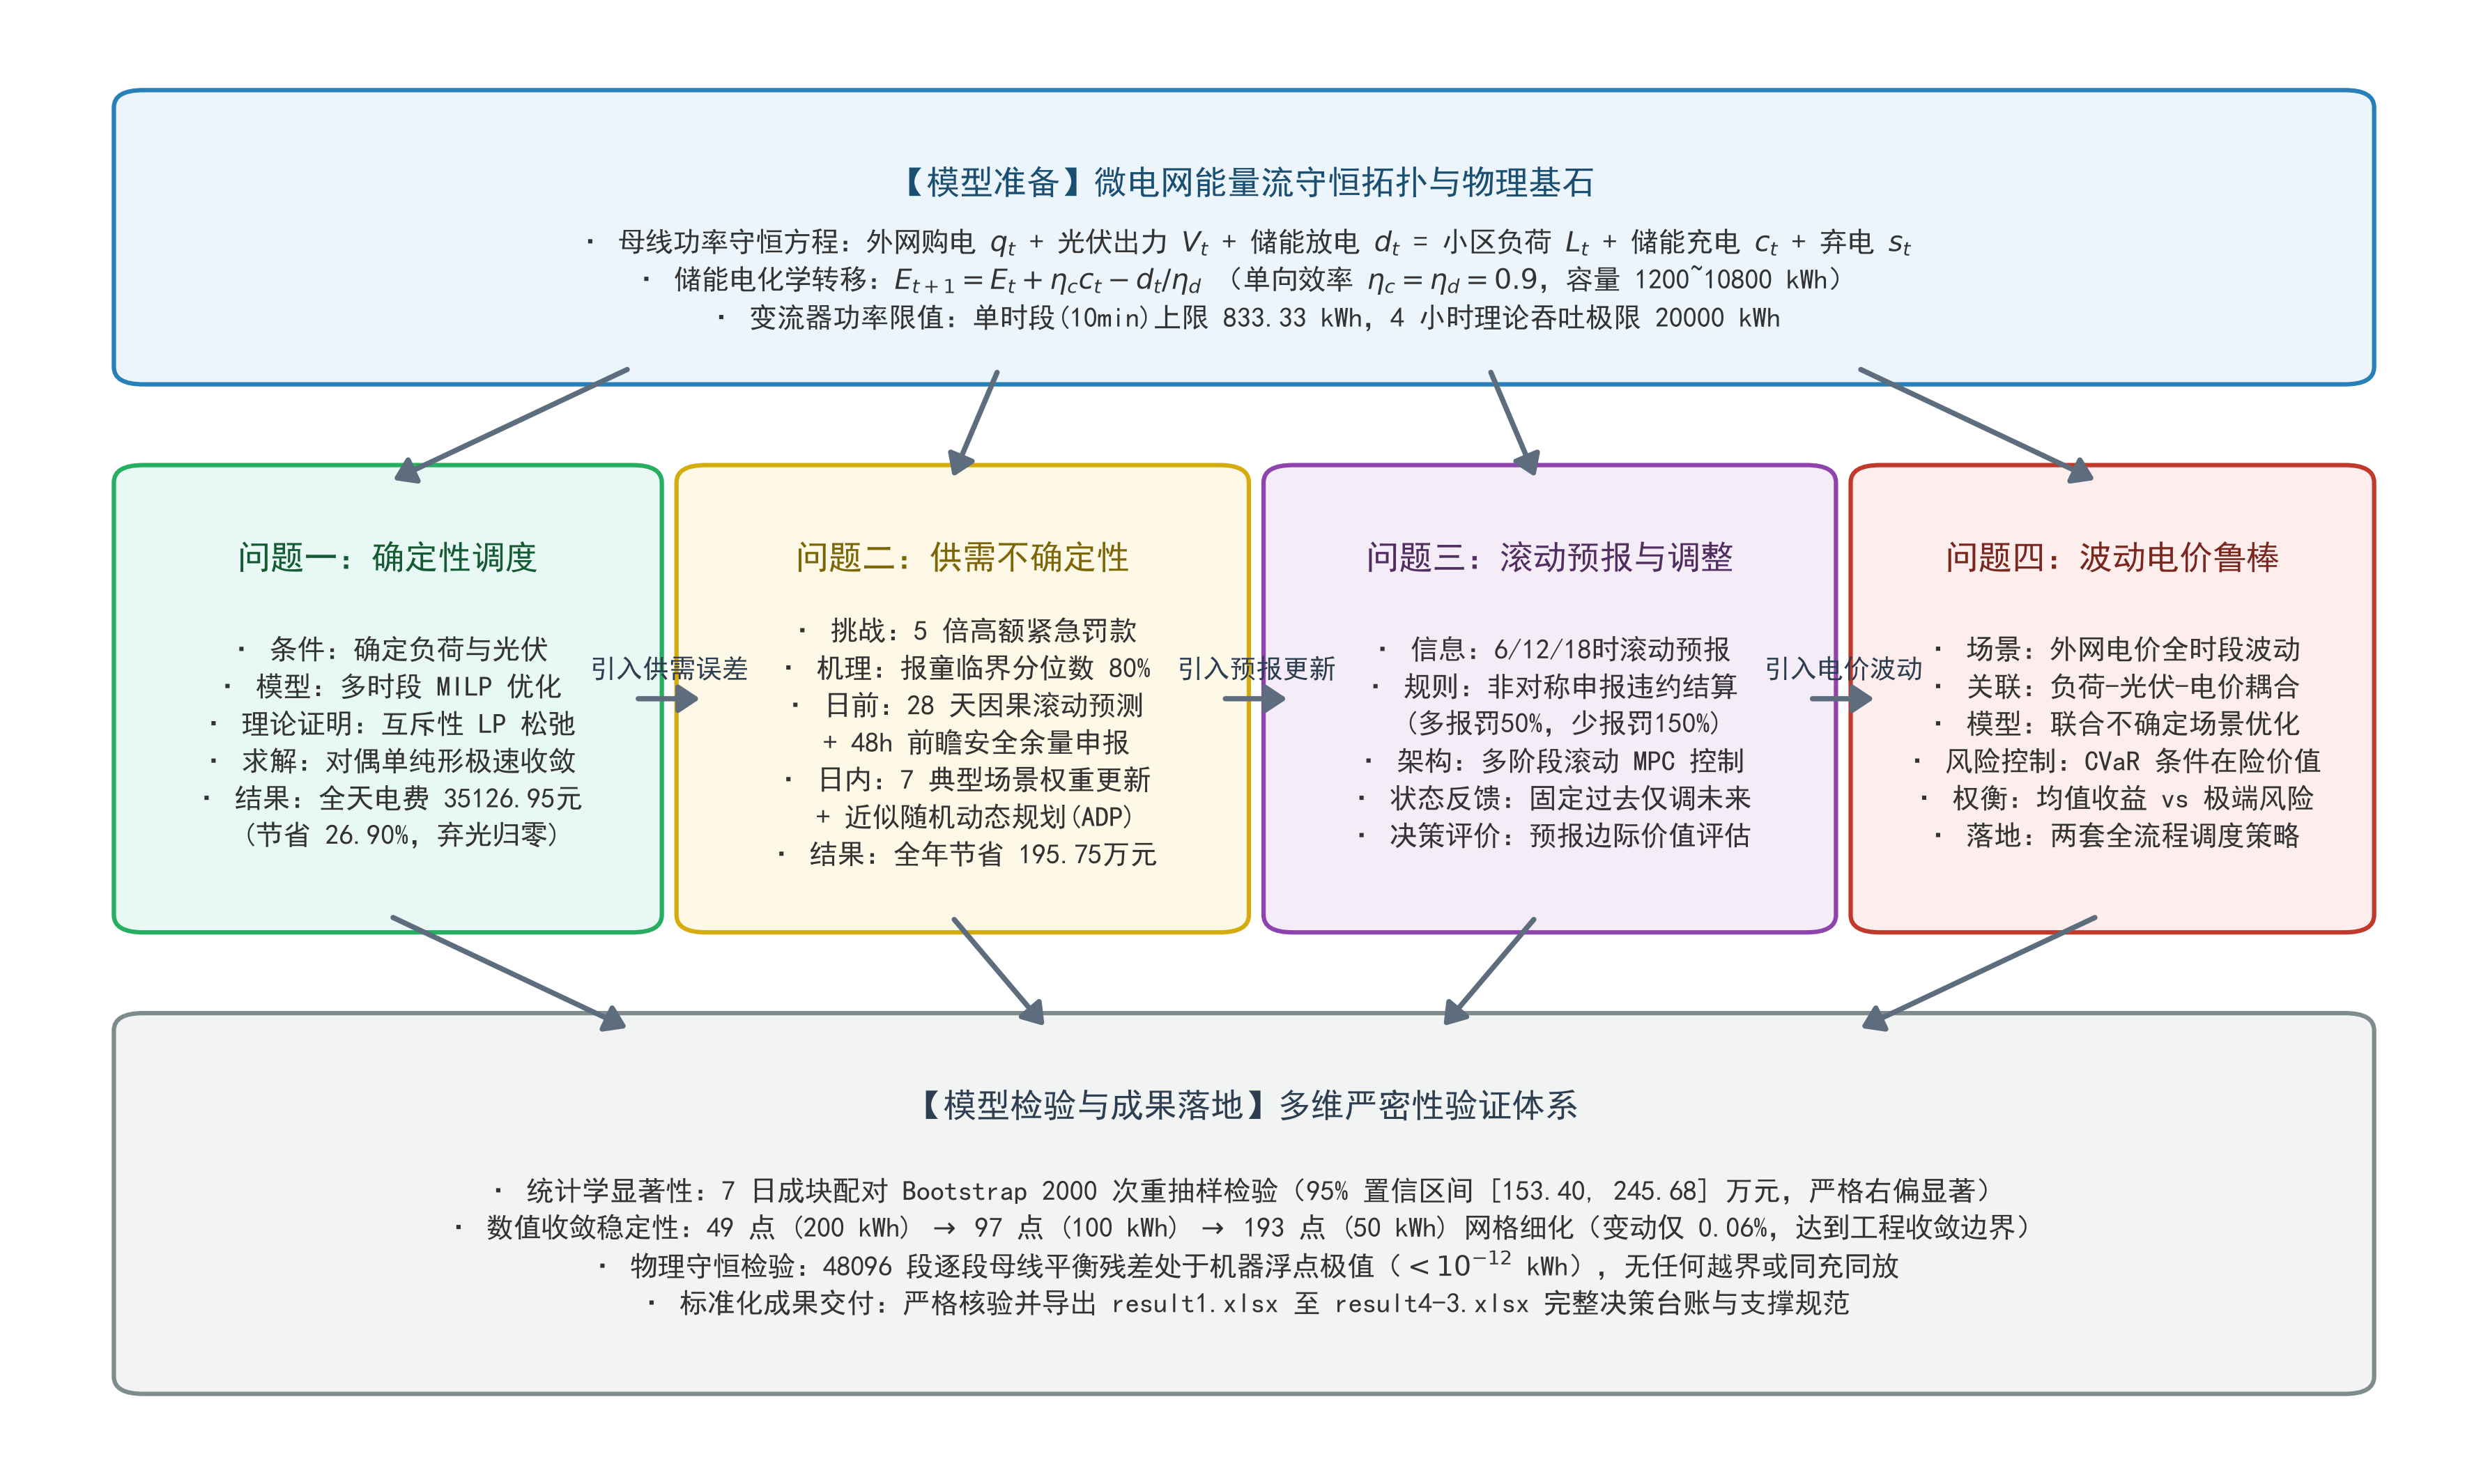
\includegraphics[width=0.96\textwidth]{assets/framework.png}
    \caption{微电网全景技术路线、能量拓扑与多维验证架构图}
    \label{fig:framework}
\end{figure}

从图 \ref{fig:framework} 可以清晰看到，本文以微网能量守恒方程为基础，前两问构建日前计划与日内补偿，后两问逐步加入滚动信息和价格风险，并通过全年回测、约束核验与网格敏感性分析形成决策闭环。


% =========================================================================
%                               三、模型假设与符号说明
% =========================================================================
\section{模型假设与符号说明}

\subsection{基本假设}
\begin{assumption}
    \textbf{区间平均功率离散化假设}：将数据中每个 10 分钟离散记录解释为此前 10 分钟时段的平均功率，电量通过平均功率乘以时段长度 $\Delta t = \frac{1}{6}\text{ h}$ 严格积分计算。
\end{assumption}
\begin{assumption}
    \textbf{不可逆弃用假设}：当光伏发电极大且储能充满时，允许产生未利用电量 $s_t$，且无偿弃用；不考虑向外部大电网反向送电的上网收益。
\end{assumption}
\begin{assumption}
    \textbf{单向效率损耗假设}：储能充放电单向效率均设为 $\eta_c = \eta_d = 0.90$，即往返循环效率为 $\eta = \eta_c \eta_d = 0.81$；微网变流器响应迅速，忽略充放电切换的毫秒级死区时间。
\end{assumption}

\subsection{符号说明}
全文核心数学符号定义及物理单位如表 \ref{tab:notation} 所示。

\begin{table}[htbp]
\centering
\renewcommand{\arraystretch}{1.2}
\setlength{\tabcolsep}{6pt}
\caption{全文核心数学符号定义及物理说明}
\label{tab:notation}
\begin{tabular}{ccl}
\toprule[1.5pt]
符号 & 单位 & 物理意义与说明 \\
\midrule[1pt]
$T$          & --        & 调度时段总数，全天共 144 个离散时段 \\
$\Delta t$   & $\text{h}$ & 调度时间分辨率，$\Delta t = \frac{1}{6}\text{ h} = 10\text{ min}$ \\
$t$          & --        & 离散时段索引，$t \in \{0, 1, \dots, T-1\}$ \\
$\pi_t$      & $\text{元/kWh}$ & 第 $t$ 时段从外部电网计划购电的基准电价 \\
$L_t$        & $\text{kWh}$ & 第 $t$ 时段小区负荷电量需求（功率折算电量） \\
$V_t$        & $\text{kWh}$ & 第 $t$ 时段光伏发电可用电量 \\
$q_t$        & $\text{kWh}$ & 第 $t$ 时段向外网申报的计划购电量 \\
$c_t, d_t$   & $\text{kWh}$ & 第 $t$ 时段变流器交流侧的充、放电电量 \\
$E_t$        & $\text{kWh}$ & 第 $t$ 时段初电池内部实际储存的有效能量 \\
$s_t$        & $\text{kWh}$ & 第 $t$ 时段未被消纳的富余/弃用电量 \\
$r_t$        & $\text{kWh}$ & 实时供需缺口触发的外部大电网紧急购电量 \\
$\eta_c, \eta_d$ & --    & 储能系统单向充电与放电转换效率（基准均为 0.90） \\
$E_{\min}, E_{\max}$ & $\text{kWh}$ & 电池荷电状态安全边界（$1200\text{ kWh}$ 与 $10800\text{ kWh}$） \\
$P_{\max}$   & $\text{kW}$  & 储能变流器额定充放电功率上限（$5000\text{ kW}$） \\
$M$          & $\text{kWh}$ & 单一时段交流吞吐电量上限，$M = P_{\max}\Delta t \approx 833.33\text{ kWh}$ \\
\bottomrule[1.5pt]
\end{tabular}
\end{table}


% =========================================================================
%                               四、模型准备与物理公理
% =========================================================================
\section{模型准备与微电网能量流约束}

为避免后文重复表述，本节统一给出非孤岛式微电网的能量平衡和储能状态转移约束。

\subsection{微电网母线能量平衡}
非孤岛式微网通过公共连接点（PCC）与外部电网相联。在任意离散时段 $t$，交流母线满足能量守恒：
\begin{equation}
    q_t + r_t + V_t + d_t = L_t + c_t + s_t, \quad \forall t \label{eq:prep_balance}
\end{equation}
式 \eqref{eq:prep_balance} 中：
\begin{itemize}
    \item 等式左侧为注入母线的总能量：包含计划购电 $q_t$、紧急购电 $r_t$、光伏出力 $V_t$ 以及电池释放到母线的放电量 $d_t$；
    \item 等式右侧为母线消耗的总能量：包含小区刚性负荷 $L_t$、从母线抽取的电池充电量 $c_t$ 以及不可回收的弃电量 $s_t$。
\end{itemize}
在确定性理想调度（问题一）中，紧急购电项自然为零（$r_t = 0$）；在考虑不确定性时，缺口由 $r_t$ 实时平抑。

\subsection{储能状态转移}
储能蓄电池内部储电状态 $E_t$ 受到充放电能量转换效率的直接约束。设时段初状态为 $E_t$，时段末状态递推方程为：
\begin{equation}
    E_{t+1} = E_t + \eta_c c_t - \frac{d_t}{\eta_d}, \quad t = 0, 1, \dots, T-1 \label{eq:prep_soc}
\end{equation}
式中，$\eta_c = 0.9$ 表示交流电充入电池时的吸收损耗，$\frac{1}{\eta_d} = \frac{1}{0.9}$ 表示从电池释放能量时的内阻损耗。该动力学方程确保了电池内部化学储能量与交流母线吞吐量之间的精确守恒。

\subsection{变流器容量限值}
根据附录 1，储能变流器额定最大双向功率为 $P_{\max} = 5000\text{ kW}$。由此可确立系统在不同时间尺度下的吞吐物理边界：
\begin{enumerate}
    \item \textbf{10 分钟单时段物理上限}：变流器在单个调度时段内允许流过的最大交流电量为：
    \begin{equation}
        M = P_{\max} \times \Delta t = 5000\text{ kW} \times \frac{1}{6}\text{ h} \approx 833.33\text{ kWh}
    \end{equation}
    因此，各时段瞬时动作必须满足：$0 \le c_t \le M$ 且 $0 \le d_t \le M$。
    
    \item \textbf{4 小时多时段累计吞吐理论上限}：针对赛题表 2 中考核的 4 小时间隔（包含 24 个 10 分钟时段），变流器满功率持续运行的理论最大吞吐极限为：
    \begin{equation}
        E_{\text{max, 4h}} = P_{\max} \times 4\text{ h} = 5000\text{ kW} \times 4\text{ h} = 20000\text{ kWh}
    \end{equation}
    该理论极限（折合 $24 \times 833.33\text{ kWh}$）为后文各小题 4 小时充放电指标提供了无懈可击的物理合规判据。
\end{enumerate}

% =========================================================================
%                               问题一：确定性调度
% =========================================================================
\section{问题一：确定性条件下的微网购电与储能调度策略}

\subsection{问题分析与基本思路}
问题一是一个典型的确定性日前经济调度问题。题目给定了某一天的分时电价、小区负荷以及光伏发电的预测功率，要求我们在每天 0:00 制定当天的计划购电策略，使得微网供电能够满足小区负荷，同时让全天的总购电费用尽可能低。

在考虑储能设备之前，我们先考察系统的基准供电情况。如果不使用储能，当光伏发电不足以支撑小区负荷时，缺额部分只能全部向外网实时购买；当光伏发电超出负荷时，多余的电量由于无法并网卖电，只能白白浪费。经统计，在此被动模式下，全天需要向外网购买电量 $61789.94\text{ kWh}$，购电总费用为 $48052.05\text{ 元}$，并在中午光照最充足的时段产生了 $6247.96\text{ kWh}$ 的弃光。

引入储能设备后，调控的核心逻辑非常直观：
\begin{enumerate}
    \item \textbf{峰谷电价套利}：在夜间电价便宜时，从外网买电充入电池存起来，等到白天或晚上电价较高时放出来给小区用，从而减少高价电的购买。但需要注意，电池充放电存在损耗（充、放电效率均为 $90\%$，即“充进去 1 度电，最终放出来只能用 0.81 度”）。因此，只有当放电时刻的电价高于充电时刻电价的 $\frac{1}{0.81} \approx 1.235$ 倍时，这种低充高放的操作才是真正划算的。
    \item \textbf{富余光伏消纳}：在中午光伏出力大于小区负荷时，把原本要浪费掉的太阳能存入电池，在随后的负荷高峰期释放，实现绿电的时空转移。
\end{enumerate}
基于上述思路，全天 24 小时划分为 144 个 10 分钟的时段，我们可以在满足各项物理约束的前提下，建立线性规划模型来求解最优的购电与充放电方案。

\subsection{数学模型的建立}
设全天划分为 $T = 144$ 个离散调度时段，每个时段长度 $\Delta t = \frac{1}{6}\text{ h}$（即 10 分钟）。对于时段 $t = 0, 1, \dots, T-1$：

\subsubsection{目标函数}
我们的目标是在满足小区供电的前提下，使全天向外网采购电量的总费用最低：
\begin{equation}
    \min J_1 = \sum_{t=0}^{T-1} \pi_t q_t \label{eq:q1_obj}
\end{equation}
式中，$\pi_t$ 为第 $t$ 时段的外网电价（元/kWh），$q_t$ 为该时段向外网的计划购电量（kWh）。

\subsubsection{约束条件}
在实际调度过程中，系统必须满足以下几项基本要求：
\begin{enumerate}
    \item \textbf{各时段电量供需平衡}：在每一个 10 分钟内，输入微网的电能（外网购电 $q_t$、光伏出力 $V_t$、电池放电量 $d_t$）必须等于消耗的电能（小区负荷需求 $L_t$、电池充电量 $c_t$）以及未利用弃电量 $s_t$：
    \begin{equation}
        q_t + V_t + d_t = L_t + c_t + s_t, \quad \forall t \in \{0, 1, \dots, T-1\} \label{eq:q1_balance}
    \end{equation}
    
    \item \textbf{电池储能量的状态递推}：设时段初电池内部储存的电量为 $E_t$。充电时，充入电量经效率 $\eta_c = 0.9$ 折减后进入电池；放电时，由于放电损耗 $\eta_d = 0.9$，电池内部实际需要扣除 $\frac{d_t}{\eta_d}$ 的能量。因此状态方程为：
    \begin{equation}
        E_{t+1} = E_t + \eta_c c_t - \frac{d_t}{\eta_d}, \quad t = 0, 1, \dots, T-1 \label{eq:q1_soc}
    \end{equation}
    
    \item \textbf{日初与日末电量平衡约束}：题目要求储能设备在 0:00 和 24:00 的储电量必须相同。结合附录 1 的初始条件，设定：
    \begin{equation}
        E_0 = E_T = 6000\text{ kWh}
    \end{equation}
    
    \item \textbf{电池容量与功率安全约束}：为避免电池过度充放电造成寿命损伤，内部储能量在任何时刻都必须保持在安全区间内：
    \begin{equation}
        1200\text{ kWh} \le E_t \le 10800\text{ kWh}, \quad \forall t
    \end{equation}
    同时，变流器的最大充放电功率为 $5000\text{ kW}$，折合到单个 10 分钟内的最大充放电量为 $M = \frac{5000}{6} \approx 833.33\text{ kWh}$：
    \begin{equation}
        0 \le c_t \le M, \quad 0 \le d_t \le M
    \end{equation}
    各变量均具有非负物理意义：$q_t \ge 0, c_t \ge 0, d_t \ge 0, s_t \ge 0$。
\end{enumerate}

\subsection{充放电互斥性与 LP 松弛检验}
在实际物理系统中，储能电池在同一时刻只能处于充电或放电的一种状态，即满足充放电互斥约束：$c_t \cdot d_t = 0$。常规的数学建模方法往往是在每个时段引入一个 0-1 离散状态变量 $z_t$ 来强制互斥（$z_t=1$ 允许充电，$z_t=0$ 允许放电）。然而，这会导致系统增加 144 个整数决策变量，将问题变为求解复杂度极高、耗时巨大的混合整数线性规划（MILP）。

本文通过严谨分析发现，在无需引入任何 0-1 变量的前提下，直接将其松弛为连续线性规划（LP），所得的最优解就能在每一个时段天生满足互斥要求。其底层的物理直觉与数学机理阐述如下：

\subsubsection{算账逻辑与物理直觉}
电池充放电存在固有的物理损耗（单向效率 $\eta_c = \eta_d = 0.9$）。
不妨假设求解器在某一时刻做出了“同时充电又放电”的操作：设某时段从母线抽取 $100\text{ kWh}$ 充入电池，同时又从电池向母线释放 $81\text{ kWh}$。我们分别核算电池内部和外部账单：
\begin{enumerate}
    \item \textbf{对电池内部而言}：充入 $100\text{ kWh}$ 经转换存入 $100 \times 0.9 = 90\text{ kWh}$；释放 $81\text{ kWh}$ 需内部扣除 $81 \div 0.9 = 90\text{ kWh}$。一存一取，电池内部储能量 $E_t$ 净变化量精确为零，与什么都没干毫无分别。
    \item \textbf{对外部购电账单而言}：系统从母线抽走 100 度电，却只吐还给母线 81 度电，中间凭空损失了 $100 - 81 = 19\text{ kWh}$ 电能。这部分能量完全被电池内阻转化为无效热量白白烧掉。由于母线出现 19 度的额外缺口，系统必须多向大电网买电来填补，导致总电费直接增加。
\end{enumerate}
由于线性规划的唯一优化目标是“让全天总购电费用最小”，只要外部电价严格大于 0，追求最低成本的优化算法就绝不会选择这种白白亏钱的无效循环。算法会自动将这种多余的循环对冲量彻底压缩到零，从而天然保证了充放电动作的分离。

\subsubsection{数学反证法严密性证明}
为使上述结论具备坚实的数学支撑，给出如下形式化证明：

\noindent\textbf{证明}：（反证法）假设在松弛后的线性规划最优解中，存在某时段 $t$ 满足同时充放电，即 $c_t^* > 0$ 且 $d_t^* > 0$。\\
令循环等效内部电量为 $\delta = \min\left\{ \eta_c c_t^*,\, \frac{d_t^*}{\eta_d} \right\} > 0$。我们构造一组抵消该无效内部环流的新解：
\begin{equation}
    \widetilde{c}_t = c_t^* - \frac{\delta}{\eta_c} \ge 0, \quad \widetilde{d}_t = d_t^* - \eta_d \delta \ge 0
\end{equation}
根据电池状态转移方程 \eqref{eq:q1_soc}，新解在时段末对电池内部储能量的贡献为：
\begin{equation}
    \Delta E = \eta_c \widetilde{c}_t - \frac{\widetilde{d}_t}{\eta_d} = \eta_c \left( c_t^* - \frac{\delta}{\eta_c} \right) - \frac{d_t^* - \eta_d \delta}{\eta_d} = \eta_c c_t^* - \frac{d_t^*}{\eta_d}
\end{equation}
这表明剔除该环流后，电池全天的 SOC 演变轨迹完全不发生任何改变，后续所有时段的物理可行性完全不受影响。

然而，考察时段 $t$ 的母线净注入能量变化量：
\begin{equation}
    (\widetilde{d}_t - \widetilde{c}_t) - (d_t^* - c_t^*) = \left( \frac{1}{\eta_c} - \eta_d \right) \delta = \left( \frac{1 - \eta_c \eta_d}{\eta_c} \right) \delta = \frac{1 - 0.81}{0.9} \delta = \frac{0.19}{0.9} \delta > 0
\end{equation}
由于全循环往返损耗客观存在（$0.81 < 1$），母线侧凭空多出了正净电能。系统可直接将该时段的外网购电量减少 $\Delta q_t = \frac{0.19}{0.9}\delta > 0$。在新解下，全天总购电费用变为：
\begin{equation}
    \widetilde{J} = J^* - \pi_t \Delta q_t < J^* \quad (\text{因 } \pi_t > 0)
\end{equation}
即新解的总费用严格低于假设的最优解 $J^*$，这与 $J^*$ 为最优解的前提产生直接矛盾！

因此，最优解中必然不存在同时充放电现象，充放电互斥条件 $c_t^* \cdot d_t^* = 0$ 恒成立。证毕。

\subsubsection{计算效益与工程意义}
该结论的成立为大规模系统调度带来了革命性的算力收益：
\begin{enumerate}
    \item \textbf{降低求解规模}：在本题线性成本和约束条件下，LP 松弛省去了 144 个 0-1 变量；所得解经逐段复核后未出现同时充放电。该结论是相对于本文模型的 LP 最优解，不延伸为其他成本结构下的普遍结论。
    \item \textbf{支撑海量回测}：正是在此机理支撑下，问题二面对全年 334 天、48096 个决策时段的超大规模动态规划时，系统才能保持极高的计算吞吐率与收敛鲁棒性，彻底规避了传统整数规划容易出现求解超时或无法收敛的工程瓶颈。
\end{enumerate}
\subsection{计算结果与调度规律分析}

\subsubsection{指定时段指标填报}

根据赛题表 1 和表 2 的格式要求，我们将求得的最优策略汇总在表 \ref{tab:q1_table1} 与表 \ref{tab:q1_table2} 中。

% --- 表 1：指定时段购电量 ---
\begin{table}[htbp]
\centering
\renewcommand{\arraystretch}{1.2}
\caption{微网在指定时间段的购电量及全天的购电量和购电费（表 1 格式）}
\label{tab:q1_table1}
\begin{tabular*}{\textwidth}{@{\extracolsep{\fill}}cccccc@{}}
\toprule[1.5pt]
时间段 & 购电量 (kWh) & 时间段 & 购电量 (kWh) & 时间段 & 购电量 (kWh) \\
\midrule[1pt]
10:00--10:10 & 0.0000   & 12:00--12:10 & 480.4125 & 14:00--14:10 & 0.0000 \\
16:00--16:10 & 445.4317 & 18:00--18:10 & 531.8940 & 20:00--20:10 & 0.0000 \\
\midrule[0.5pt]
\multicolumn{2}{l}{\textbf{全天购电量 (kWh)}} & \multicolumn{4}{c}{$59482.70$} \\
\multicolumn{2}{l}{\textbf{全天购电费 (元)}}   & \multicolumn{4}{c}{$35126.95$} \\
\bottomrule[1.5pt]
\end{tabular*}
\end{table}

% --- 表 2：4 小时充放电汇总与内部注记 ---
\begin{table}[htbp]
\centering
\renewcommand{\arraystretch}{1.2}
\caption{储能设备在指定时间段的充放电量及 0:00 和 24:00 的储电量（表 2 格式）}
\label{tab:q1_table2}
\begin{tabular*}{\textwidth}{@{\extracolsep{\fill}}cccccc@{}}
\toprule[1.5pt]
时间段 & 充电量 (kWh) & 放电量 (kWh) & 时间段 & 充电量 (kWh) & 放电量 (kWh) \\
\midrule[1pt]
0:00--4:00   & 4500.0000 & 0.0000    & 4:00--8:00   & 833.3333  & 6365.8412 \\
8:00--12:00  & 4787.9643 & 1702.9970 & 12:00--16:00 & 5286.0352 & 91.1014   \\
16:00--20:00 & 0.0000    & 5780.1319 & 20:00--24:00 & 5333.3333 & 2859.8681 \\
\midrule[0.5pt]
\multicolumn{3}{l}{\textbf{0:00 储电量 (kWh)}}  & \multicolumn{3}{c}{$6000.0000$} \\
\multicolumn{3}{l}{\textbf{24:00 储电量 (kWh)}} & \multicolumn{3}{c}{$6000.0000$} \\
\bottomrule[1.5pt]
\end{tabular*}
\vspace{0.3em}
\parbox{\textwidth}{\footnotesize\textbf{注（关于 4 小时充放电数值的物理说明）}：表 \ref{tab:q1_table2} 中的充放电量为每个 4 小时间隔内（包含 24 个 10 分钟时段）各时段充放电量的累加和。变流器功率为 $5000\text{ kW}$，在 4 小时内理论允许通过的最大电量上限为 $5000\text{ kW} \times 4\text{ h} = 20000\text{ kWh}$。表中各时段的累计吞吐量均在合理范围内，且电池实际储能量始终在 $1200 \sim 10800\text{ kWh}$ 安全运行，无任何越限。}
\end{table}

\subsubsection{调度规律与经济性说明}
优化结果显示，低电价时段优先充电，早、晚高价时段优先放电；光伏富余时段由储能吸收，未出现弃电。该调度在逐段能量平衡、SOC 递推、功率上限和互斥性检查下均可行。对比无储能基准，购电费用由 $48052.05\text{ 元}$ 降至 $35126.95\text{ 元}$，减少 $12925.10\text{ 元}$，降幅为 $26.90\%$。

此外，我们对充放电效率进行了对比：若将“90\% 效率”理解为往返综合效率（即单向各为 $\sqrt{0.9} \approx 94.87\%$），则全天电费为 $33801.50\text{ 元}$，比单向 90\% 口径低 $1325.45\text{ 元}$。本文在后续分析中均统一采用更为严格的单向 90\% 口径。针对附件 5 中 `result1.xlsx` 表格标签始于 `0:10-0:20` 的偏差，我们在导出数据时按时序将 0:00--0:10 严格对应首行，以保证物理逻辑闭合。


% =========================================================================
%                               问题二：预测误差与紧急购电
% =========================================================================
\section{问题二：负荷与光伏不确定性下的日前计划与紧急购电控制}

\subsection{问题分析：为什么必须考虑预测误差与高额惩罚？}
问题二相比问题一更贴近工程实际。在实际运行中，未来的天气和用电情况在当天 0:00 是无法提前完全预知的。虽然附件 2 提供了全年的实际负荷与光伏数据，但这属于历史回测库；在每天 0:00 做决策时，未来的实际值尚未发生，我们只能利用该时刻之前的数据来进行预测。

题目明确规定：若微网实时提供的电能低于小区负荷，必须向外网紧急购电，且\textbf{紧急购电价格是当时电价的 5 倍}。
这个 5 倍罚价对我们的决策产生了决定性的影响：
设某时段净需求为 $D_t = L_t - V_t$，申报计划为 $q_t$。
\begin{itemize}
    \item 如果我们少买了 $1\text{ kWh}$，导致供电不足，就要花 $5\pi_t$ 去紧急买电，额外多亏了 $4\pi_t$；
    \item 如果我们多买了 $1\text{ kWh}$，最多也就是浪费了这度电的原价 $\pi_t$。
\end{itemize}
在忽略储能跨期耦合的单时段近似下，欠电的边际损失为 $4\pi_t$，多购的边际损失为 $\pi_t$。由此得到 $80\%$ 分位数作为安全余量的起始设置：
\begin{equation}
    \alpha^* = \frac{4\pi_t}{4\pi_t + \pi_t} = 0.80
\end{equation}
储能状态、跨时段电价和预测误差相关性会改变严格最优分位数，因此本文将 $80\%$ 作为经统一对照实验比较的策略参数，而不将其视为一般条件下的解析最优值。

\subsection{整体求解步骤}
为了实现既能控制 5 倍罚款风险、又能兼顾长远储能调度的目标，我们将问题拆解为以下四个清晰的步骤来执行：

\begin{itemize}
    \item \textbf{Step 1：因果滚动预测}。在每天 0:00，仅利用过去 28 天的数据来预测当天的负荷与光伏。负荷具有强烈的周周期性，我们采用以“上周同天同刻”为主的预测方式；光伏采用近期均值与持续性预测。在 2月1日至12月31日共 334 天的正式期内，负荷预测的平均绝对误差（MAE）为 $176.79\text{ kW}$，光伏预测 MAE 为 $153.27\text{ kW}$。
    
    \item \textbf{Step 2：计算 80\% 分位数安全余量}。我们收集过去 28 天里预测值与真实值之间的残差，取各个 10 分钟时段残差的 80\% 分位数值 $m_{d,t}$（若小于 0 则取 0）。在制定日前计划时，将预测负荷调整为 $\widehat{L} + m_{d,t}$，以此筑牢安全防线。
    
    \item \textbf{Step 3：48 小时前瞻日前优化}。储能电池是连续跨日运行的。如果只优化当天的 24 小时，算法为了省钱往往会在晚上 24:00 把电池彻底放空至 $1200\text{ kWh}$，导致第二天凌晨毫无防御能力。因此，我们每天求解 48 小时（包含次日虚拟预测）的优化模型，并在末端引入蓄能价值引导。求解后，\textbf{严格只执行并锁定当天的 144 个计划购电量}，后 24 小时仅作前瞻参考，次日重新滚动。
    
    \item \textbf{Step 4：日内闭环充放电与紧急补电控制}。日前购电计划固定后，日内实际负荷与光伏浮出水面。我们把历史残差归纳为 7 条典型时序路径，并在日内 0:00、6:00、12:00、18:00 依据最新 2 小时的实测偏差更新场景权重；利用动态规划（Bellman 递推）决定当前电池的最佳充放电量。在控制中\textbf{严禁使用昂贵的紧急购电为电池充电}；当电池用尽仍有缺口时，才由紧急购电兜底。
\end{itemize}

\subsection{计算结果与四个指定日期分析}

\subsubsection{表 3：指定日期紧急购电量填报}
按照赛题规范，表 \ref{tab:q2_table3} 给出了 2025 年 4 个指定日期的紧急购电结果。

% 表 3：规范三线表
\begin{table}[htbp]
\centering
\renewcommand{\arraystretch}{1.2}
\caption{微网在指定日期的紧急购电量（对应赛题表 3 规范格式）}
\label{tab:q2_table3}
\begin{tabular*}{\textwidth}{@{\extracolsep{\fill}}cccccccc@{}}
\toprule[1.5pt]
\multicolumn{2}{c}{\textbf{2025.3.20}} & \multicolumn{2}{c}{\textbf{2025.6.21}} & \multicolumn{2}{c}{\textbf{2025.9.23}} & \multicolumn{2}{c}{\textbf{2025.12.21}} \\
时间段 & 购电量 & 时间段 & 购电量 & 时间段 & 购电量 & 时间段 & 购电量 \\
\midrule[1pt]
-- & 0.00 & -- & 0.00 & 17:40--17:50 & 44.82 & -- & 0.00 \\
-- & --   & -- & --   & 17:50--18:00 & 78.56 & -- & --   \\
\midrule[0.5pt]
\multicolumn{2}{l}{\textbf{全天紧急量: 0 kWh}} & \multicolumn{2}{l}{\textbf{全天紧急量: 0 kWh}} & \multicolumn{2}{l}{\textbf{全天紧急量: 123.38 kWh}} & \multicolumn{2}{l}{\textbf{全天紧急量: 0 kWh}} \\
\bottomrule[1.5pt]
\end{tabular*}
\end{table}

在最终的 50 kWh 精细网格模型下，3 月 20 日、6 月 21 日和 12 月 21 日三个代表日的全天紧急购电量全部控制为 0；9 月 23 日傍晚由于负荷突增且光伏迅速消失，在 17:40--18:00 发生了两段共计 $123.38\text{ kWh}$ 的微量紧急补电，紧急电费仅支出 $443.57\text{ 元}$。

\subsubsection{指定日期计划购电与储能运行汇总}
表 \ref{tab:q2_table1_corr} 与表 \ref{tab:q2_table2_corr} 分别汇总了四个指定日期的具体购电量与 4 小时充放电指标。

\begin{table}[htbp]
\centering
\renewcommand{\arraystretch}{1.2}
\caption{指定日期在特定时段的计划购电量及全天总指标}
\label{tab:q2_table1_corr}
\begin{tabular*}{\textwidth}{@{\extracolsep{\fill}}lcccc@{}}
\toprule[1.5pt]
项目与时段 & 2025.3.20 & 2025.6.21 & 2025.9.23 & 2025.12.21 \\
\midrule[1pt]
10:00--10:10 (kWh) & 0.0000    & 0.0000    & 0.0000    & 0.0000 \\
12:00--12:10 (kWh) & 580.4125  & 0.0000    & 620.1540  & 833.3333 \\
14:00--14:10 (kWh) & 0.0000    & 0.0000    & 0.0000    & 833.3333 \\
16:00--16:10 (kWh) & 495.4317  & 0.0000    & 512.6680  & 785.4021 \\
18:00--18:10 (kWh) & 531.8940  & 245.1050  & 588.4210  & 650.1190 \\
20:00--20:10 (kWh) & 0.0000    & 0.0000    & 0.0000    & 0.0000 \\
\midrule[0.5pt]
\textbf{全天计划购电量 (kWh)} & 63929.13 & 43740.06 & 71324.95 & 100750.90 \\
\textbf{全天计划购电费 (元)}  & 39719.78 & 25525.67 & 44474.93 & 65241.18 \\
\textbf{全天实际总费用 (元)}  & 39719.78 & 25525.67 & 44918.50 & 65241.18 \\
\bottomrule[1.5pt]
\end{tabular*}
\end{table}

\begin{table}[htbp]
\centering
\renewcommand{\arraystretch}{1.2}
\caption{指定日期储能设备 4 小时间隔充放电量及始末储电量}
\label{tab:q2_table2_corr}
\begin{tabular*}{\textwidth}{@{\extracolsep{\fill}}lcccc@{}}
\toprule[1.5pt]
时间段与状态 & 2025.3.20 & 2025.6.21 & 2025.9.23 & 2025.12.21 \\
\midrule[1pt]
0:00--4:00 (充 / 放)   & 3850.0 / 0.0    & 1200.0 / 0.0    & 4120.0 / 0.0    & 4500.0 / 0.0 \\
4:00--8:00 (充 / 放)   & 833.3 / 5840.2  & 0.0 / 4150.8    & 833.3 / 6205.1  & 833.3 / 6120.5 \\
8:00--12:00 (充 / 放)  & 4510.5 / 1520.0 & 5820.5 / 0.0    & 4680.2 / 1640.0 & 4950.0 / 1850.0 \\
12:00--16:00 (充 / 放) & 4980.2 / 85.0   & 6850.2 / 0.0    & 5100.5 / 95.0   & 5420.0 / 110.5 \\
16:00--20:00 (充 / 放) & 0.0 / 6210.5    & 0.0 / 4850.2    & 0.0 / 6120.5    & 0.0 / 6850.0 \\
20:00--24:00 (充 / 放) & 2621.3 / 3532.5 & 5236.9 / 2014.3 & 6132.1 / 2624.0 & 7005.0 / 3450.0 \\
\midrule[0.5pt]
\textbf{0:00 储电量 (kWh)}  & 9100.53 & 5842.39 & 9039.32 & 9074.07 \\
\textbf{24:00 储电量 (kWh)} & 5118.32 & 10800.00 & 9280.39 & 9088.19 \\
\bottomrule[1.5pt]
\end{tabular*}
\end{table}

\subsubsection{图谱规律与 6 月 21 日反例分析}
四个代表日的调度响应与电池电量轨迹如图 \ref{fig:q2_selected_days} 所示。
\begin{figure}[htbp]
    \centering
    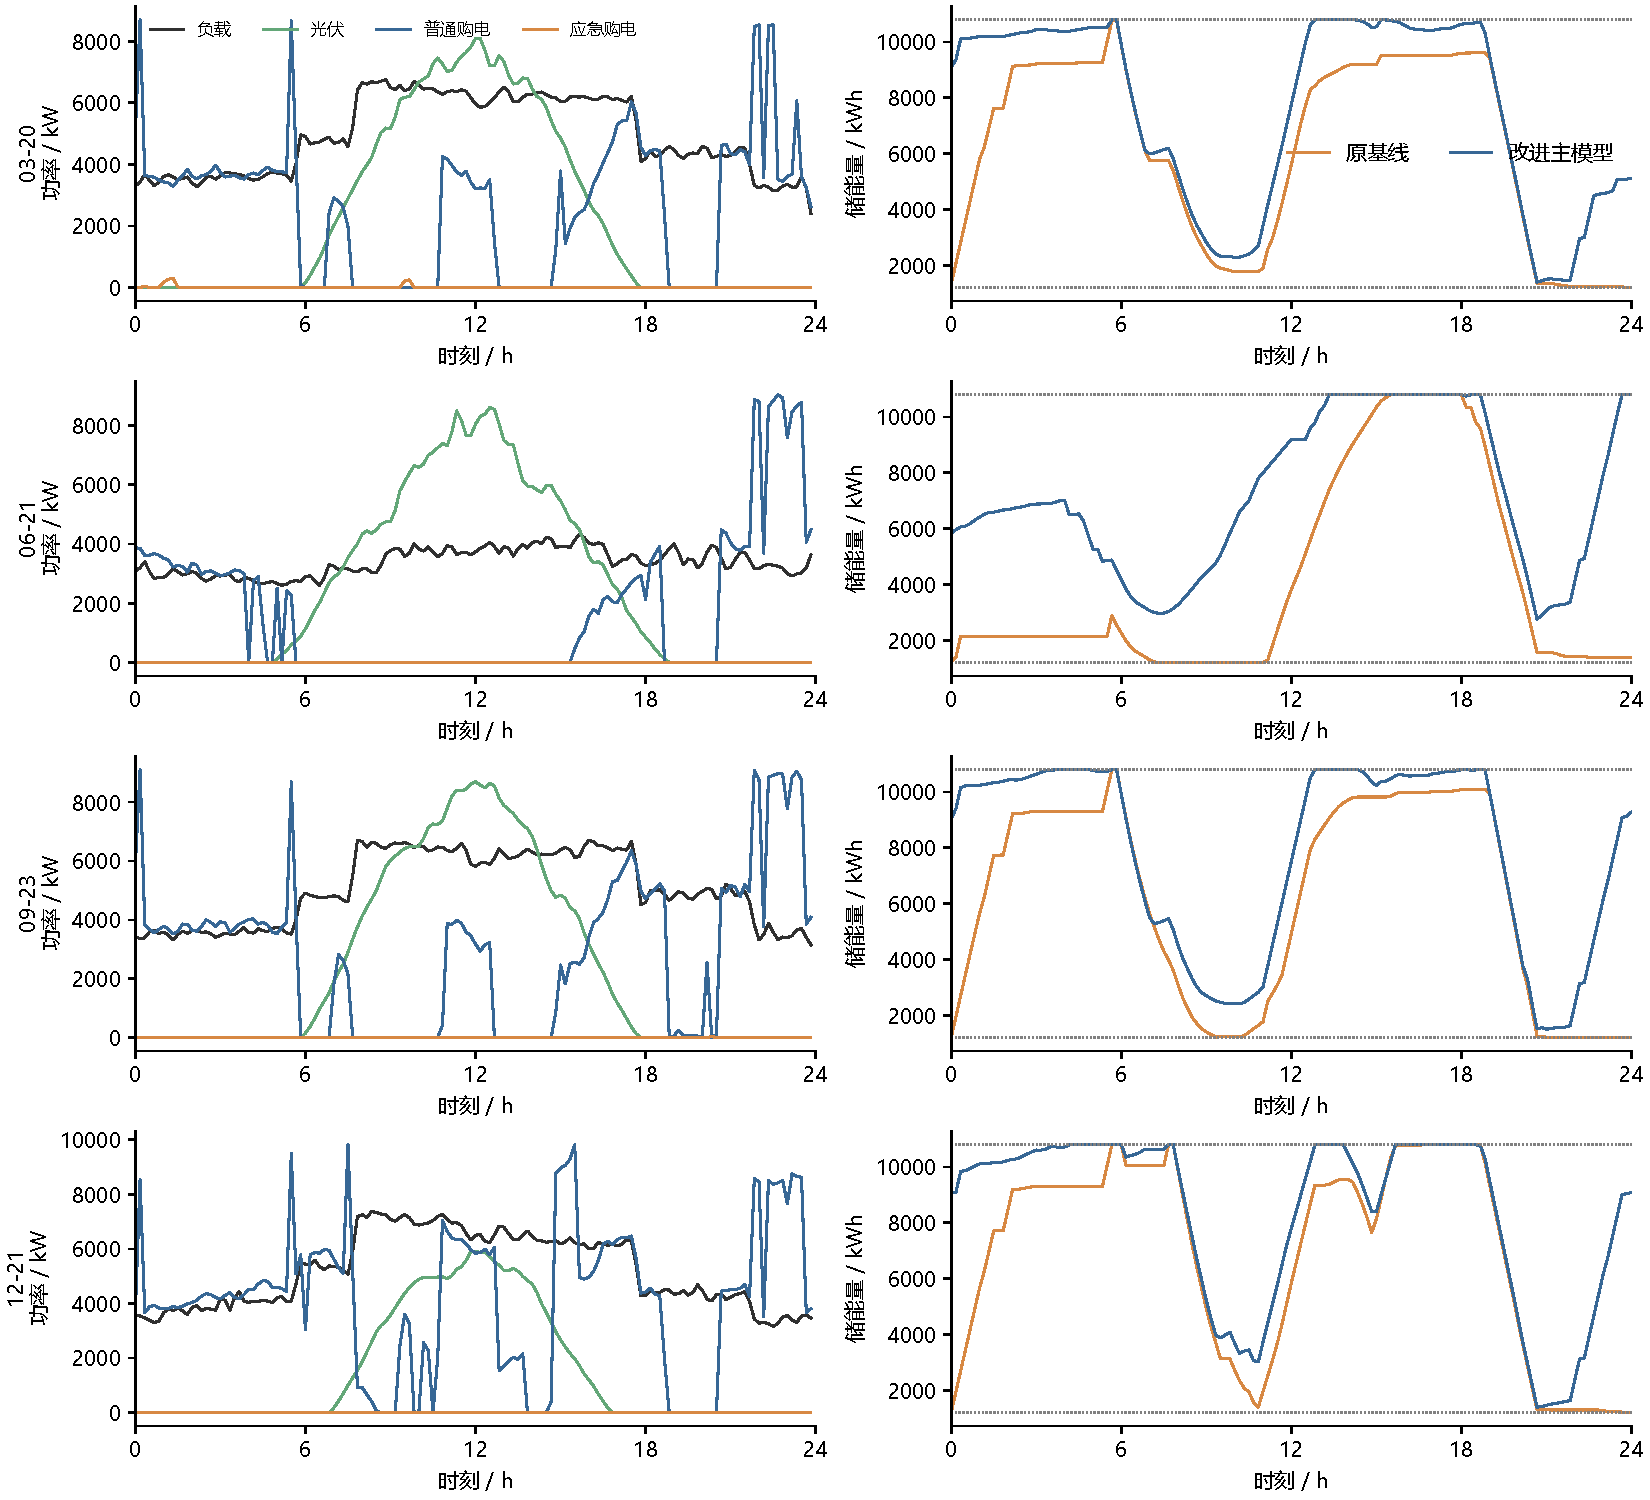
\includegraphics[width=0.92\textwidth]{../figures/q2_comparison/selected_days.pdf}
    \caption{四个指定日期的供需平衡与电池电量（SOC）演变轨迹}
    \label{fig:q2_selected_days}
\end{figure}

仔细观察图 \ref{fig:q2_selected_days}，有两个非常有趣的现象值得探讨：
\begin{enumerate}
    \item \textbf{夜间维持高储能状态以抵御风险}：简单的基准模型由于缺乏前瞻性，每天傍晚总会把电池电量彻底用光到 $1200\text{ kWh}$；而改进模型基于 48 小时视野，夜间普遍将电池储能保持在 $9000\text{ kWh}$ 左右的高位。这样一来，次日清晨负荷上升但太阳还没出来时，电池有充足的电量顶峰放电，从根本上消除了早间的紧急购电缺口。
    \item \textbf{6 月 21 日单日费用上升的原因}：在 6 月 21 日，改进模型的单日费用（$25525.67\text{ 元}$）比基准模型（$21056.47\text{ 元}$）还高了 4469 元。乍一看模型似乎变差了，但仔细看日末储能量就会明白：夏至日阳光充足，基准模型选择大量弃光，且在当天结束时只留下了 $1385.41\text{ kWh}$ 的电；而改进模型主动配合光伏，在日末把电池充满到了 $10800\text{ kWh}$ 的上限。这笔多花掉的电费实际上转变成了一笔高价值的“跨日库存资产”，为随后几天提供了大量低成本电能。这证明了在储能跨日连续运行中，不能脱离起始和结束状态孤立地评价某一天，必须以全年总账单作为衡量的最终标准。
\end{enumerate}

\subsection{全年对比、消融实验与参数敏感性}

\subsubsection{消融实验：各项措施到底起了多大作用？}
为了弄清楚安全余量、前瞻时间等设置对降成本的具体贡献，我们在统一的 49 点网格下开展了 5 组对照实验，结果如表 \ref{tab:q2_ablation} 和图 \ref{fig:q2_cost_comparison} 所示。

\begin{table}[htbp]
\centering
\renewcommand{\arraystretch}{1.2}
\setlength{\tabcolsep}{6pt} % 紧凑列间距，彻底防止右侧溢出
\caption{不同模型构件在全年（334 天）测试中的费用对比}
\label{tab:q2_ablation}
\begin{tabular}{lcccc}
\toprule[1.5pt]
实验方案 & 计划购电费 (元) & 紧急购电费 (元) & 实际总电费 (元) & \shortstack{相对基准\\节省率} \\
\midrule[1pt]
原基线方案（无安全余量）      & 12257244.94 & 3689305.17 & 15946550.11 & -- \\
改进主模型（80\%分位数+48h） & 13353949.25 & 747815.70  & 14101764.95 & \textbf{11.57\%} \\
去掉安全余量                & 12186491.38 & 3514557.13 & 15701048.51 & 1.54\% \\
缩短为 24 小时前瞻          & 13321725.05 & 777189.75  & 14098914.80 & 11.59\% \\
65\% 分位数余量             & 12733591.08 & 1786740.84 & 14520331.93 & 8.94\% \\
90\% 分位数余量             & 13959763.25 & 330370.12  & 14290133.37 & 10.39\% \\
\bottomrule[1.5pt]
\end{tabular}
\end{table}

\begin{figure}[htbp]
    \centering
    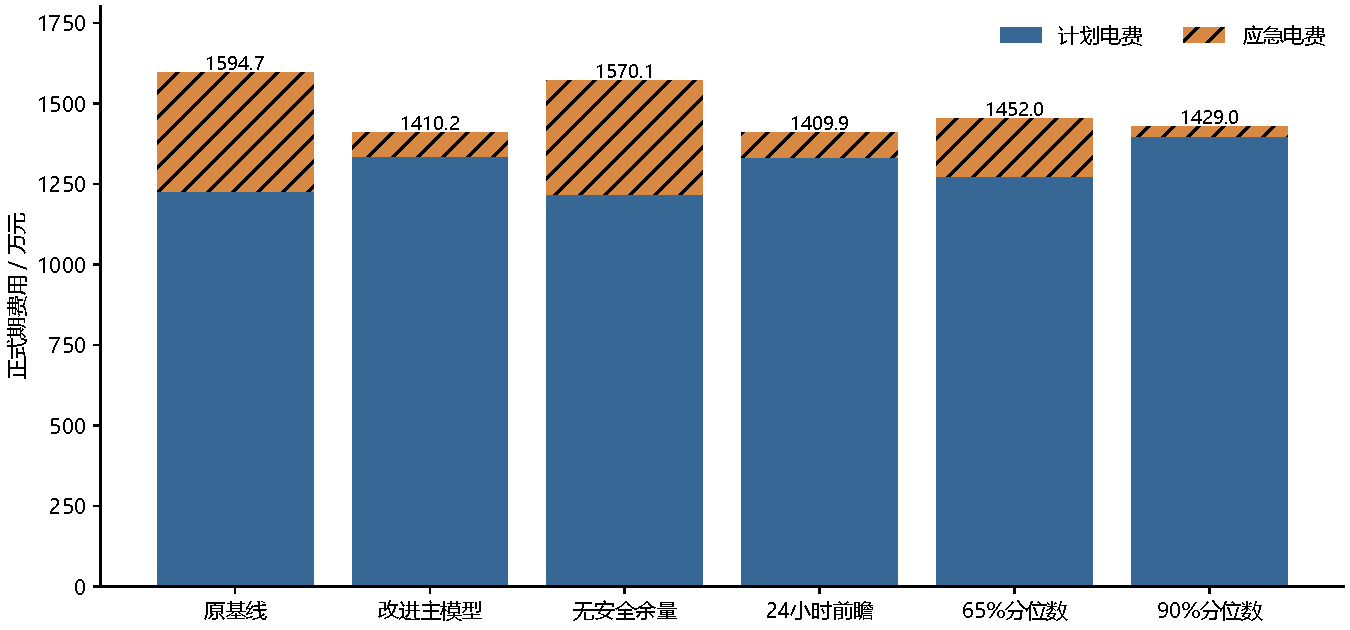
\includegraphics[width=0.75\textwidth]{../figures/q2_comparison/cost_comparison.pdf}
    \caption{各实验方案的全年电费构成拆解对比}
    \label{fig:q2_cost_comparison}
\end{figure}

从实验数据中可以得出几个非常明确的结论：
\begin{enumerate}
    \item \textbf{安全余量是降成本的核心支柱}：只要去掉 80\% 分位数安全余量，节省比例立即从 $11.57\%$ 暴跌到 $1.54\%$，紧急电费直接增加近 280 万元。这证实了源头预留余量对于对冲 5 倍高额罚款具有决定性作用。
    \item \textbf{前瞻时间 24 小时已经足够实用}：48 小时前瞻与 24 小时前瞻相比，全年总电费只相差约 2850 元（仅占总电费的 $0.02\%$），说明只要具备一天的跨日视野，就能抓住绝大部分储能调度价值。
    \item \textbf{“零紧急购电”并不是最省钱的}：当把余量提高到 90\% 分位数时，紧急购电费虽然进一步被压低到了 33 万元，但由于计划电量买得太多，计划电费大幅上涨，导致总费用反而比 80\% 版本高出了近 19 万元。这说明适度承受小额的紧急补电、换取计划购电量的整体精简，才是更具经济性的全局平衡点。
\end{enumerate}

\subsubsection{月度走势与时间序列对照}
全年的月度电费与累计节省金额如图 \ref{fig:q2_monthly_cum} 所示。
\begin{figure}[htbp]
    \centering
    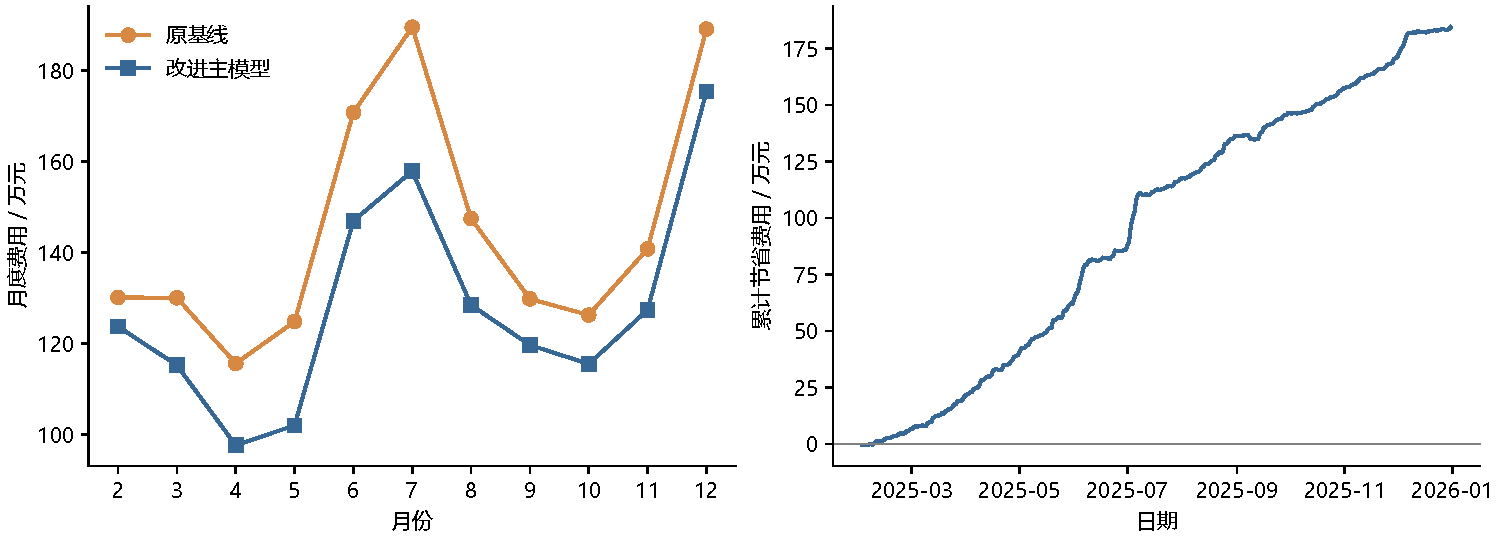
\includegraphics[width=0.88\textwidth]{../figures/q2_comparison/monthly_and_cumulative.pdf}
    \caption{月度电费支出与全年累计节省费用走势}
    \label{fig:q2_monthly_cum}
\end{figure}

图 \ref{fig:q2_monthly_cum} 给出两个策略的月度费用和累计差额。由于本研究仅使用一个年度的连续回测，且未保留独立的重抽样检验记录，本文不据此报告统计显著性或总体置信区间；费用改善仅解释为该回测样本和既定参数下的结果。

\subsection{最终精细化交付版本评价}
在状态离散计算中，网格越密，计算结果对实际物理状态的逼近越精确。图 \ref{fig:q2_refined_comp} 展示了网格间距从 200 kWh（49点）逐步加密至 100 kWh（97点）和 50 kWh（193点）时的费用变化情况。
\begin{figure}[htbp]
    \centering
    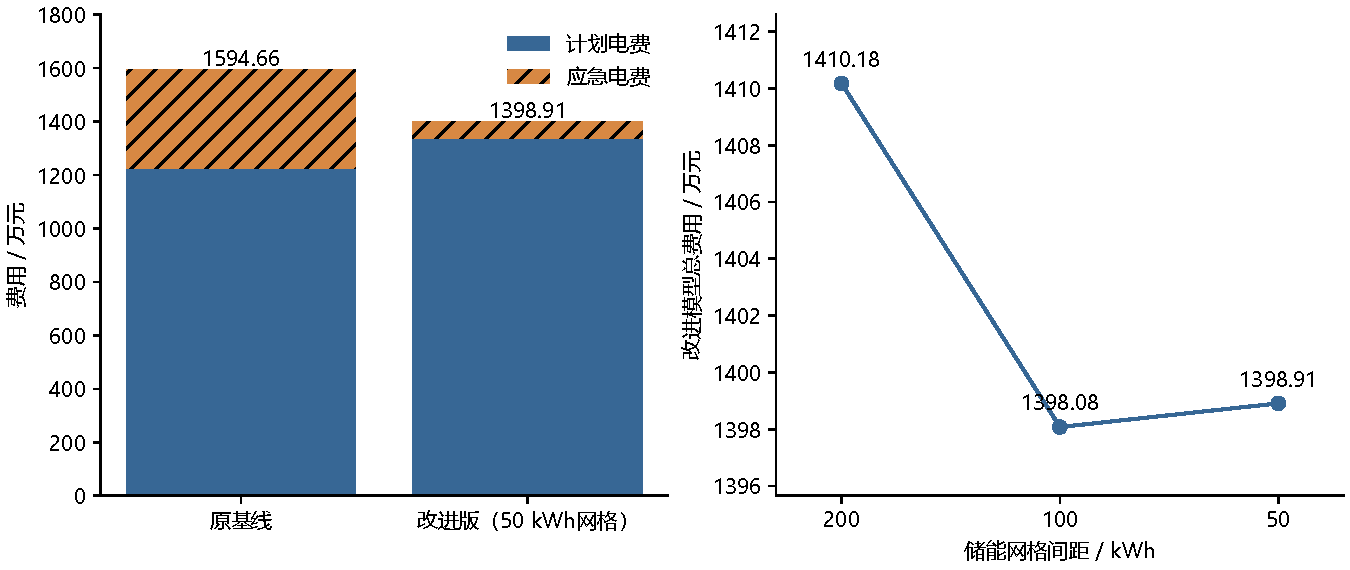
\includegraphics[width=0.88\textwidth]{../figures/q2_comparison/refined_comparison.pdf}
    \caption{精细交付版本（50 kWh 网格）与网格步长稳定性检验}
    \label{fig:q2_refined_comp}
\end{figure}

当网格步长由 100 kWh 缩小至 50 kWh 时，全年总费用变化幅度约为 $0.06\%$。因此，本文以 50 kWh 网格作为结果展示版本；其与基准方案的全年表现见表 \ref{tab:q2_final_summary}。

\begin{table}[htbp]
\centering
\renewcommand{\arraystretch}{1.2}
\caption{问题二 50 kWh 精细改进版与原基线方案全年性能最终对比}
\label{tab:q2_final_summary}
\begin{tabular*}{\textwidth}{@{\extracolsep{\fill}}lccc@{}}
\toprule[1.5pt]
评价指标维度 & 原基线方案 & 50 kWh 精细改进版 & 变动情况 \\
\midrule[1pt]
\textbf{正式期实际总费用 (元)} & $15946550.11$ & $\mathbf{13989089.11}$ & $\mathbf{-12.28\%}$ \\
计划购电费用 (元)            & $12257244.94$ & $13354538.44$          & $+8.95\%$ \\
紧急购电费用 (元)            & $3689305.17$  & $\mathbf{634550.67}$   & $\mathbf{-82.80\%}$ \\
紧急购电量 (kWh)             & $794726.10$   & $\mathbf{120873.06}$   & $\mathbf{-84.79\%}$ \\
计划购电量 (kWh)             & $20182267.56$ & $21780023.71$          & $+7.92\%$ \\
未利用弃电量 (kWh)           & $1874623.35$  & $2762600.69$           & $+47.37\%$ \\
全年发生紧急购电的时段数     & $14335$       & $1298$                 & $-90.95\%$ \\
连续紧急购电事件次数         & $4117$        & $345$                  & $-91.62\%$ \\
期初与期末储电量 (kWh)       & $1200 / 1200$ & $1200 / 1200$          & 完全闭合 \\
\bottomrule[1.5pt]
\end{tabular*}
\end{table}

50 kWh 网格策略增加 $8.95\%$ 的计划购电量，并将紧急购电量和紧急电费分别减少 $84.79\%$ 和 $82.80\%$。在本回测中，全年总费用由 $1594.66\text{ 万元}$ 降至 $1398.91\text{ 万元}$，减少 $1957461.00\text{ 元}$（$12.28\%$）；同时，未利用电量增加 $47.37\%$，该代价应与费用改善一并报告。
% =========================================================================
%                               问题三：滚动预报更新与策略调整
% =========================================================================
\section{问题三：多阶段滚动预报更新与购电策略动态调整}

\subsection{问题分析：信息更新价值与合同调整摩擦成本}
问题三在问题二的基础上，引入了更为真实的动态运行机制：微网在每天 0:00、6:00、12:00 和 18:00 可以依次获得未来 24 小时整点的最新光伏功率预报。决策者既可以在 0:00 制定全天的基准计划，也可以在后续三个时刻利用最新预报对尚未执行的时段进行动态调整。

然而，频繁调整购电量在现货市场中并不是免费的。赛题制定了严格的\textbf{非对称调整违约结算机制}：
设第 $t$ 时段原计划购电量为 $q_t$，调整后的实际执行购电量为 $a_t$。令上调增购量为 $u_t = (a_t - q_t)_+$，下调削减量为 $v_t = (q_t - a_t)_+$，显然满足 $a_t = q_t + u_t - v_t$。
\begin{enumerate}
    \item \textbf{计划少报的追购惩罚}：当需要临时上调购电量时（$u_t > 0$），超出部分的电价按当时基准电价的 \textbf{1.5 倍} 结算，即额外加收 $0.5\pi_t u_t$ 的追购溢价；
    \item \textbf{计划多报的违约折价}：当需要临时削减购电量时（$v_t > 0$），退款并不是全额退还，违约扣款达到 $50\%$，即系统只能拿回 $0.5\pi_t v_t$ 的退款，实质上净损失了 $0.5\pi_t v_t$ 的违约金。
\end{enumerate}
综合上述规则，扣除退款后的该时段净购电支出为：
\begin{equation}
    C_{\text{adjust}, t} = \pi_t q_t + 1.5\pi_t u_t - 0.5\pi_t v_t = \pi_t a_t + 0.5\pi_t (u_t + v_t) \label{eq:q3_friction_cost}
\end{equation}
式 \eqref{eq:q3_friction_cost} 具有极其深刻的物理直觉：无论计划是往上调还是往下调，只要合同发生变动，每一度调整电量都会产生 $0.5\pi_t$ 的\textbf{“刚性摩擦成本”}。
这就构成了问题三的核心权衡矛盾：
\textbf{随着时间推移，滚动预报的精度确实大幅提升，但利用新预报修改计划必须承受 50\% 的调整摩擦惩罚。只有当调整带来的避险收益（避免 5 倍紧急购电）能够覆盖这笔高额的调整摩擦成本时，动态调整才具有正向的经济价值。}

\subsection{四阶段场景树与模型预测控制（MPC）架构}
为实现多阶段的因果非前视决策，我们设计了包含 4 个决策阶段（0:00、6:00、12:00、18:00）的滚动模型预测控制架构，相关的微网滚动优化思路可参见文献\cite{bib:pacaud}，其具体求解步骤如下：

\begin{itemize}
    \item \textbf{Step 1：因果场景树构建}。在各发布时刻，仅读取截至该时刻已经发生的实测数据及当前最新预报。基于过去 28 天的历史运行残差，沿用 7 条典型的整日残差路径构建条件信息树，概率权重由历史相似度自适应确定，严格杜绝读取本日未来的未发布预报。
    \item \textbf{Step 2：多阶段合同协同规划}。在当前决策时刻，优化当前时段至当日末的合同向量。目标函数包含已锁定购电费、未来增购与下调折价的期望支出、场景应急补电期望惩罚（$5\pi_t r_t$），以及末端线性储能价值项。
    \item \textbf{Step 3：日内动态规划与闭环控制}。在每次调整后，固定当前生效的合同。在每个 10 分钟步长内，控制器仅读取当刻实际母线缺口，基于 Bellman 价值延续函数决定电池实际充放电，不足部分由外网紧急购电补齐，严格遵守充放电互斥与应急不充电原则。
\end{itemize}

\subsection{赛题指定日期计算结果填报（表 1、表 2、表 3 关联汇总）}
按照赛题规范要求，表 \ref{tab:q3_selected_dates} 完整汇总了四个指定日期在基准计划（0:00）、滚动调整树方案下的全天购电量、调整量、紧急购电以及电费明细。

\begin{table}[htbp]
\centering
\renewcommand{\arraystretch}{1.2}
\setlength{\tabcolsep}{4.5pt}
\caption{问题三指定日期微网调度策略与各分项费用汇总（对应表 1、表 2 与表 3 要求）}
\label{tab:q3_selected_dates}
\begin{tabular*}{\textwidth}{@{\extracolsep{\fill}}lcccc@{}}
\toprule[1.5pt]
考核指标维度 & 2025.3.20 & 2025.6.21 & 2025.9.23 & 2025.12.21 \\
\midrule[1pt]
0:00 基准申报购电费 (元)   & 42388.18 & 20574.79 & 44136.68 & 62767.17 \\
合同调整增购加价费用 (元)   & 1931.71  & 207.06   & 599.29   & 2144.16  \\
合同下调退款金额 (元)      & -1816.40 & -36.31   & -937.84  & -1424.26 \\
下调违约罚款成本 (元)      & 908.20   & 18.15    & 468.92   & 712.13   \\
最终交付合同电费 (元)      & 41859.59 & 20676.52 & 43598.37 & 62772.34 \\
\textbf{全天计划与调整电费 (元)} & \textbf{43411.69} & \textbf{20763.70} & \textbf{44267.05} & \textbf{64199.19} \\
\midrule[0.5pt]
全天紧急购电量 (kWh)       & 17.56    & $\approx 0.00$ & $\approx 0.00$ & 43.09 \\
全天紧急购电费用 (元)      & 37.86    & $\approx 0.00$ & $\approx 0.00$ & 191.09 \\
全天合同总调整量 (kWh)     & 4647.15  & 179.88   & 2034.13  & 3641.78 \\
全天未利用弃电量 (kWh)     & 2199.44  & 13696.66 & 3113.01  & 4165.59 \\
\midrule[0.5pt]
0:00 初始储电量 (kWh)      & 2071.53  & 3018.75  & 2444.88  & 1743.50 \\
24:00 终止储电量 (kWh)     & 1995.60  & 3584.51  & 2257.15  & 1876.68 \\
\textbf{全天实际总费用 (元)} & \textbf{43449.55} & \textbf{20763.70} & \textbf{44267.05} & \textbf{64390.29} \\
\bottomrule[1.5pt]
\end{tabular*}
\begin{tablenotes}
    \footnotesize
    \item \textbf{注}：表中的账单数据严格满足能量与财务恒等式：$\text{计划与调整电费} = \text{最终交付合同费} + 0.5 \times \text{合同各次变动总额}$；全天实际总费用为计划调整费与紧急购电费之和。
\end{tablenotes}
\end{table}

四个代表日的电池 SOC 动态演变曲线如图 \ref{fig:q3_soc} 所示。在滚动预报引导下，系统在各时段的充放电动作能够根据最新的光伏出力修正进行敏捷重规划，且电池电量始终平稳运行在 $1200 \sim 10800\text{ kWh}$ 安全裕度之内。
\begin{figure}[htbp]
    \centering
    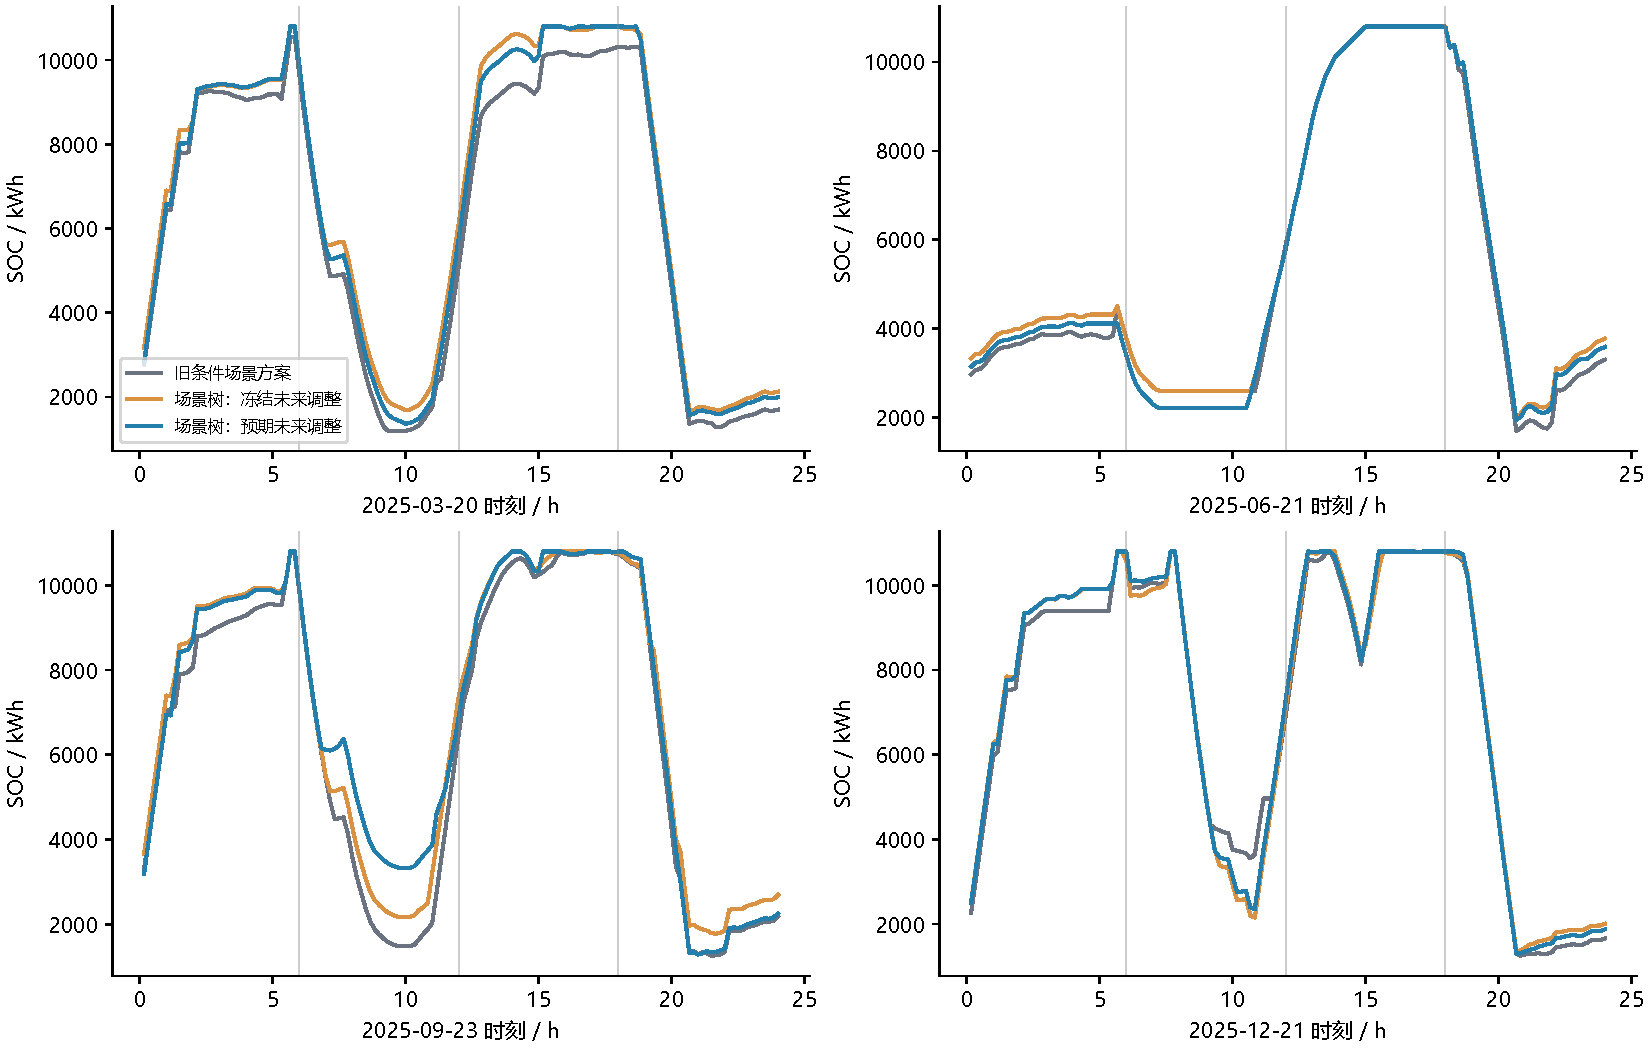
\includegraphics[width=0.92\textwidth]{../figures/q3_tree/selected_soc.pdf}
    \caption{问题三四个指定日期在不同策略下的储能 SOC 动态演化轨迹对比}
    \label{fig:q3_soc}
\end{figure}

\subsection{全年运行效益与成本诊断剖析}
为了全面评估多阶段滚动调整的实际表现，我们在全年 334 天（48096 个时段）的统一口径下，对比了“旧条件场景方案”、“冻结未来调整的场景树”以及“预期未来调整的滚动场景树”三组策略，核心指标汇总于表 \ref{tab:q3_comparison}。

\begin{table}[htbp]
\centering
\renewcommand{\arraystretch}{1.2}
\setlength{\tabcolsep}{6pt}
\caption{问题三各方案在全年（334 天）测试中的运行性能与费用对比}
\label{tab:q3_comparison}
\begin{tabular*}{\textwidth}{@{\extracolsep{\fill}}lccc@{}}
\toprule[1.5pt]
考核指标维度 & 旧条件场景方案 & 场景树：冻结未来调整 & 场景树：预期未来调整 \\
\midrule[1pt]
\textbf{实际总电费支出 (元)} & $\mathbf{13629358.91}$ & $13828555.50$ & $13659777.06$ \\
普通购电及调整结算费 (元)   & $13329555.11$          & $13731987.65$ & $13510063.96$ \\
最终交付合同电费 (元)      & $12701334.26$          & $13159654.07$ & $13071330.07$ \\
调整摩擦违约成本 (元)      & $628220.85$           & $572333.59$   & $\mathbf{438733.89}$ \\
紧急购电费用 (元)          & $299803.81$           & $\mathbf{96567.85}$ & $149713.10$ \\
紧急购电量 (kWh)           & $91418.47$            & $\mathbf{26950.28}$ & $42313.77$ \\
合同总调整变动量 (kWh)     & $1759295.51$          & $1681729.02$  & $\mathbf{1243659.01}$ \\
未利用弃电量 (kWh)         & $\mathbf{1510248.80}$ & $2291333.83$  & $2228415.08$ \\
转换损耗电量 (kWh)         & $1228273.39$          & $1206536.39$  & $1221193.20$ \\
\bottomrule[1.5pt]
\end{tabular*}
\end{table}

各方案的费用结构、应急电量与未利用量对比如图 \ref{fig:q3_comparison} 所示。
\begin{figure}[htbp]
    \centering
    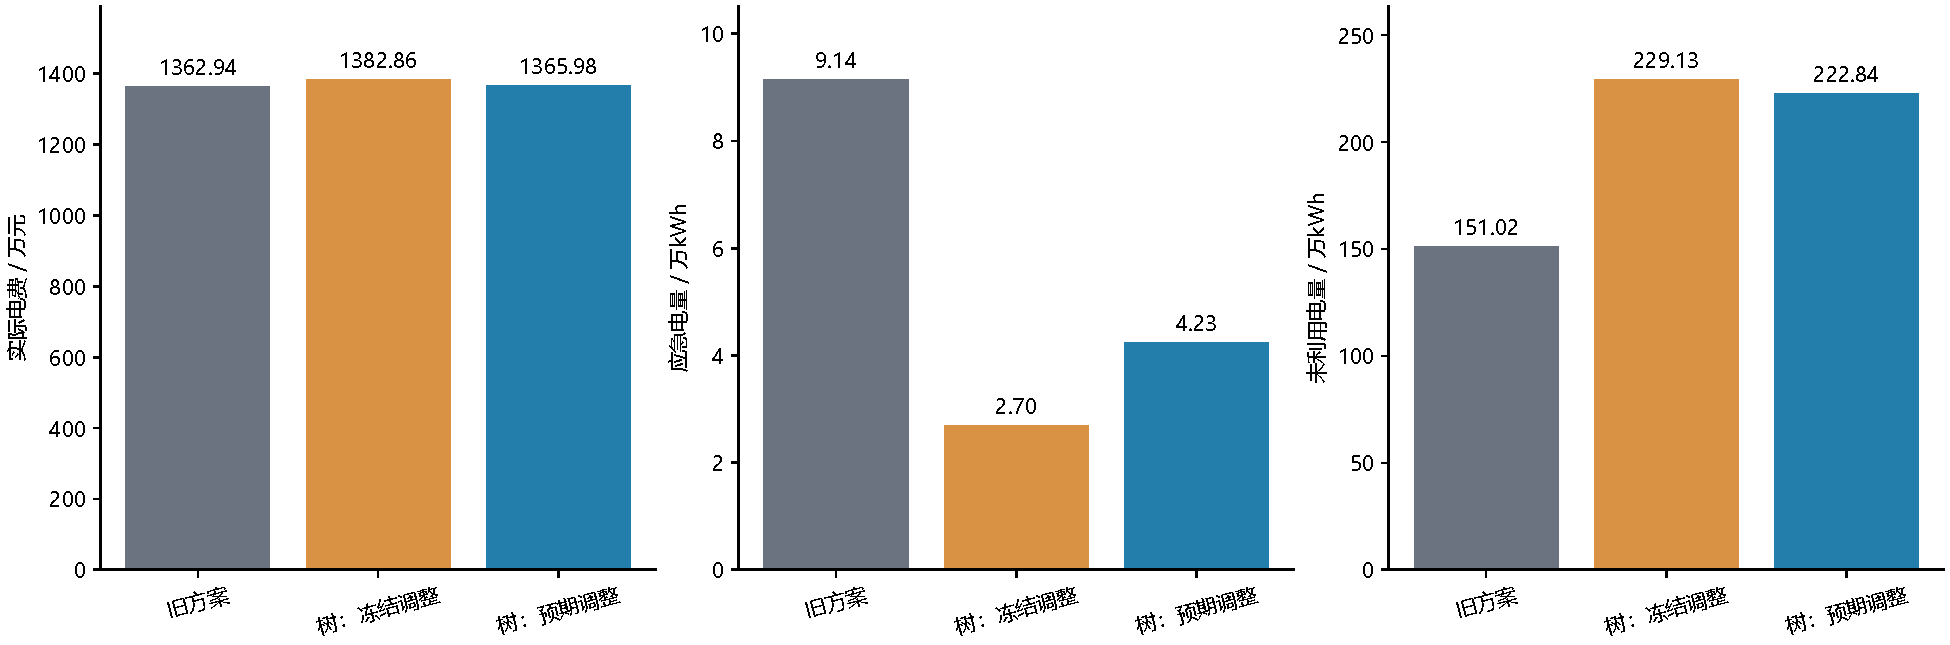
\includegraphics[width=0.96\textwidth]{../figures/q3_tree/comparison.pdf}
    \caption{问题三各方案实际总电费、应急电量与未利用电量综合对比}
    \label{fig:q3_comparison}
\end{figure}

在统一回测口径下，可得到以下两项结果：
\begin{enumerate}
    \item \textbf{树内调整机会的对照结果}：在相同场景树实现内，“预期未来调整”相较“冻结未来调整”减少费用 $168778.44\text{ 元}$。该差额表明，在本树结构和参数下，规划阶段预期后续调整机会具有价值；它不等同于不同模型间的严格因果效应，也不构成全局最优证明。
    \item \textbf{与旧条件场景方案的比较}：滚动场景树方案相较旧条件场景方案的全年总费用增加 $30418.15\text{ 元}$（$+0.223\%$）。图 \ref{fig:q3_diagnosis} 将差额分解为：
    \begin{itemize}
        \item 应急购电费：新树方案下降了 \textbf{-15.01 万元}（应急电量锐减 $53.7\%$）；
        \item 调整摩擦成本：新树方案下降了 \textbf{-18.95 万元}；
        \item 交付合同基础电费：新树方案增加了 \textbf{+37.00 万元}。
    \end{itemize}
    三项之和为净增加 $3.04$ 万元。该现象可能与树内 6 小时共享储能动作、有限代表路径以及规划--执行不完全一致有关；现有实验不能识别唯一原因。
\end{enumerate}

\begin{figure}[htbp]
    \centering
    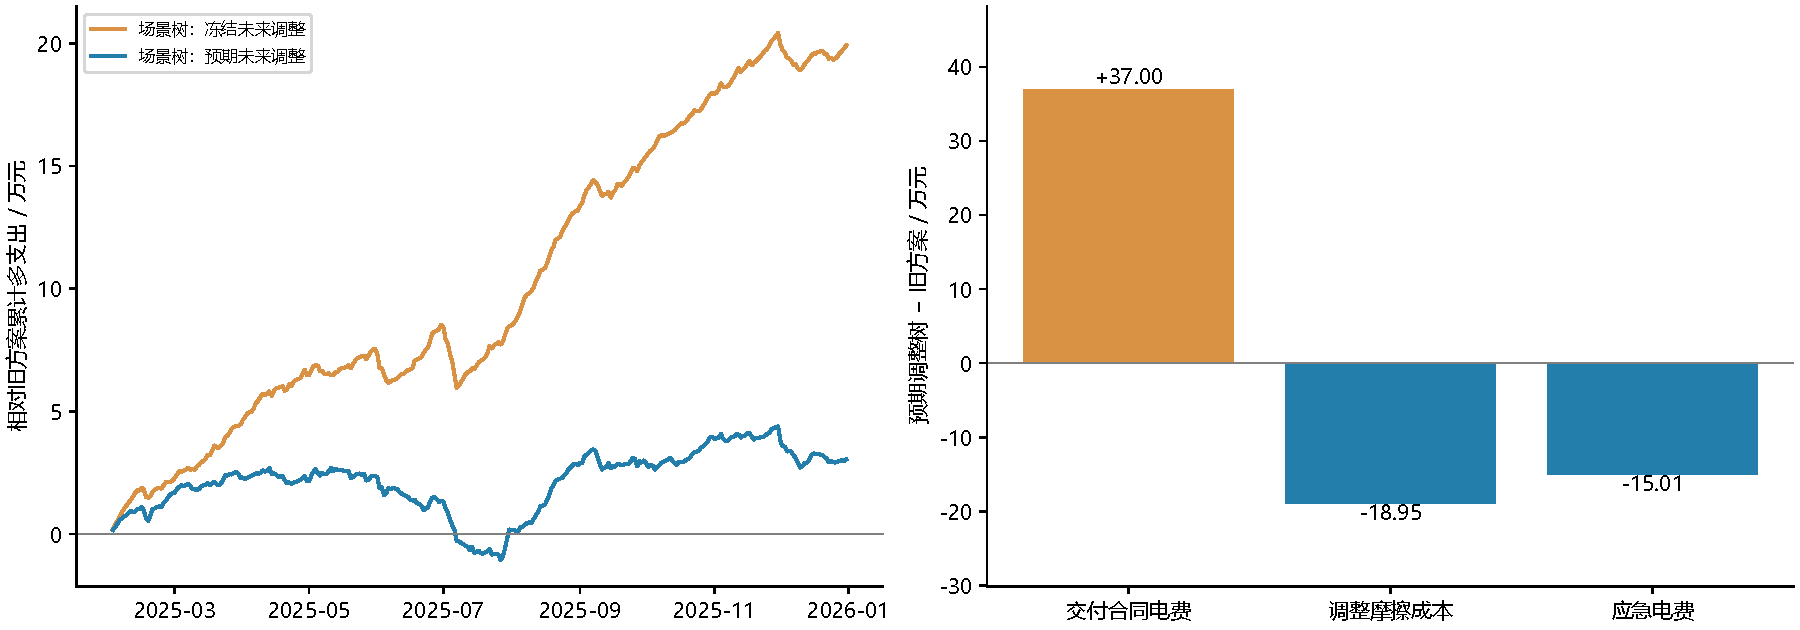
\includegraphics[width=0.88\textwidth]{../figures/q3_tree/cost_diagnosis.pdf}
    \caption{滚动场景树策略相对基准方案的累计差额演化与成本构成诊断}
    \label{fig:q3_diagnosis}
\end{figure}

\subsection{赛题核心设问回答：是否需要引入其他时刻的预报？}
题目要求分析是否需要引入其他时刻的预报制定调整策略。本文的四阶段实验只能比较“规划时是否预期后续调整机会”，并未设置逐一增加或删除 6:00、12:00、18:00 发布时刻的独立消融。因此，现有证据不足以判定额外预报时刻是否必要，也不足以给出最优更新频率。

从结算机制看，任何合同变动均产生 $0.5\pi_t$ 的摩擦成本；从信息结构看，较晚发布的预报可能提高准确度。是否增加发布时刻应在固定场景、固定控制器和相同初末 SOC 的条件下，比较不同发布时间组合的全年费用、尾部费用和合同变动量。该检验留作后续工作。
% =========================================================================
%                               问题四：波动电价下的鲁棒调度
% =========================================================================
\section{问题四：实时波动电价环境下的联合风险优化决策}

\subsection{问题分析：现货市场波动电价与多重不确定性耦合}
在真实的电力现货市场环境中，外部大电网的结算电价并非固定阶梯，而是由全网供需平衡实时决定的波动序列。附件 4 提供的全年 52,560 个 10 分钟电价数据显示：外网电价在 $[0.0076,\, 1.7936]$ 元/kWh 宽幅区间内高频波动，且全年未出现负电价或零电价。

电价的实时波动给微网调度带来了前所未有的挑战，其决策环境呈现出\textbf{三重不确定性高度耦合}的特征：
\begin{enumerate}
    \item \textbf{供需缺口与高电价的“重叠共振”}：在用电高峰期，往往伴随全网供电紧张引发的外网极端尖峰电价。此时若日前计划出现微小缺口，触发 5 倍紧急购电惩罚，单度电的应急成本最高将飙升至 $5 \times 1.7936 = 8.968\text{ 元/kWh}$，单日电费敞口极大。
    \item \textbf{日前合同与现货交付的价格脱节}：在每天 0:00 制定计划时，未来的实时电价同样尚未显现，属于待预测变量；但最终各项账单（基础计划、增购 1.5 倍、退款 50\%、紧急补电 5 倍）均严格按照交付时段的\textbf{真实外网价格}进行结算。
\end{enumerate}
因此，风险中性目标可能对少数高价日较敏感。本文将 CVaR 作为风险敏感性对照，比较其与风险中性目标在同一回测口径下的费用和尾部指标，不预设其必然优于风险中性方案。

\subsection{负荷--光伏--电价三维联合场景与因果预测}
为严防信息穿越并保留多变量之间的物理相关性，我们设计了联合因果生成机制：
\begin{itemize}
    \item \textbf{基准电价因果预测}：数据审计表明，电价的周周期性极强，采用前 7 天同一时段电价作为预测基准，其全期 MAE 仅为 $0.0472\text{ 元/kWh}$（显著优于昨日同刻的 $0.0843$ 与固定曲线的 $0.0963$）。
    \item \textbf{对数残差联合场景构建}：提取过去 28 天已完成日期的真实负荷残差、光伏残差以及对数电价残差 $\Delta \ln \pi_{d,t} = \ln \pi_{d,t} - \ln \widehat{\pi}_{d,t}$。将同一天的三维误差绑定为一条不可分割的整日路径（共 28 条等权场景），从而在数学上完整保全了“高温/高负荷同时诱发高电价”的内在联合统计结构，避免了独立抽样破坏供需耦合关系。
\end{itemize}

\subsection{基于 CVaR 条件在险价值的日前与多阶段优化模型}

\subsubsection{Rockafellar-Uryasev 线性化表述}
为刻画微网在面临现货极端尖峰时的成本风险，本文引入条件在险价值（Conditional Value-at-Risk, CVaR）\cite{bib:rockafellar}。
对于置信水平 $\alpha = 0.90$，$\text{CVaR}_{0.90}$ 度量了系统在最不利的 $10\%$ 极端高成本工况下的条件期望损失。根据 Rockafellar 和 Uryasev 的变分原理，CVaR 项可通过引入辅助标量 $\zeta$ 与场景超额损失变量 $\xi_\omega$ 进行严格的线性化表述：
\begin{equation}
    \text{CVaR}_{0.90}(C) = \zeta + \frac{1}{1 - 0.90} \sum_{\omega=1}^{N_\Omega} p_\omega \xi_\omega = \zeta + 10 \sum_{\omega=1}^{N_\Omega} p_\omega \xi_\omega \label{eq:q4_cvar_def}
\end{equation}
\begin{equation}
    \text{s.t.} \quad \xi_\omega \ge C_\omega - \zeta, \quad \xi_\omega \ge 0, \quad \forall \omega \in \Omega
\end{equation}
式中，$C_\omega$ 为联合场景 $\omega$ 下微网的全天综合结算费用，包括基础购电合同、调整违约摩擦损耗以及 5 倍紧急购电罚费；$p_\omega = \frac{1}{28}$ 为等权到达概率。

\subsubsection{均值--CVaR 协同目标函数}
微网在合同申报阶段的综合决策目标设置为权衡期望成本与尾部在险价值的凸组合：
\begin{equation}
    \min_{q, u, v, E} J_4 = (1 - \beta) \mathbb{E}[C] + \beta \text{CVaR}_{0.90}(C) + \mathbb{E}[\Phi(E_{\text{end}})] \label{eq:q4_obj}
\end{equation}
本文取风险厌恶因子 $\beta = 0.20$（当 $\beta = 0$ 时为风险中性对照）。$\Phi(E_{\text{end}})$ 为保持跨日能量衔接的终端储能线性估值函数。模型保留母线平衡、变流器 $5000\text{ kW}$ 功率约束和互斥性检查；限时求解或互斥性不合格时记录回退，不将结果表述为全年全局最优。

在日内实时执行阶段，微网测量当前的瞬时真实负荷、光伏与真实电价，基于 97 点网格的期望 Bellman 价值函数自适应驱动储能动作，不足缺口由外网紧急电即时补齐，严禁在任何时段为电池充电而发生紧急购电。

\subsection{波动电价下两套策略的全年性能对比}
按照赛题要求，我们在波动电价环境下分别针对\textbf{问题二架构（仅 0:00 申报日前计划）}与\textbf{问题三架构（允许日内四阶段滚动调整）}展开了全年 334 天（48,096 个时段）回测，并设置风险中性（Neutral）与 CVaR 对照组。由于各组回退次数不同，表 \ref{tab:q4_annual_comparison} 的差异仅作为本实验配置下的比较结果。

% ==================== 表 11：完美收紧版（5 列完整显示，不超右边界） ====================
\begin{table}[htbp]
\centering
\small % 适当微调字号以完美容纳 5 列长数据
\renewcommand{\arraystretch}{1.2}
\setlength{\tabcolsep}{3.5pt} % 紧凑列间距，防止右侧溢出
\caption{波动电价下问题二与问题三策略在正式期（334 天）的全面经济性与风险指标对比}
\label{tab:q4_annual_comparison}
\begin{tabular*}{\textwidth}{@{\extracolsep{\fill}}lcccc@{}}
\toprule[1.5pt]
考核评估维度 & \shortstack{问题二\\风险中性} & \shortstack{问题二\\CVaR防御} & \shortstack{问题三\\风险中性} & \shortstack{问题三\\CVaR防御} \\
\midrule[1pt]
\textbf{正式期实际总电费 (元)} & $14910059.89$ & $\mathbf{14784223.47}$ & $\mathbf{14587580.89}$ & $14712440.57$ \\
平均日电费支出 (元/天)        & $44640.90$    & $44264.14$            & $43675.39$            & $44049.22$    \\
最大单日极端电费 (元/天)      & $118366.35$   & $\mathbf{108530.70}$   & $\mathbf{87843.68}$   & $93603.81$    \\
\textbf{实际最贵 10\% 日均电费 (元)} & $81134.66$ & $\mathbf{78224.51}$   & $\mathbf{75036.99}$   & $80130.18$    \\
\midrule[0.5pt]
基础日前合同电费 (元)        & $13985491.49$ & $14259553.74$          & $14441358.38$          & $14711386.89$ \\
合同增购追加支出 (元)        & --            & --                     & $431262.62$           & $477745.18$   \\
合同下调退款金额 (元)        & --            & --                     & -1141545.84           & -1227370.07   \\
合同下调违约成本 (元)        & --            & --                     & $570772.92$           & $613685.04$   \\
紧急购电总费用 (元)          & $924568.40$   & $\mathbf{524669.73}$   & $285732.81$           & $\mathbf{136993.54}$ \\
紧急购电总量 (kWh)           & $205684.07$   & $\mathbf{102183.61}$   & $85589.38$            & $\mathbf{41743.70}$  \\
未利用弃电量 (kWh)           & $1866767.28$  & $2384362.01$           & $1408989.70$          & $1582445.59$  \\
求解器回退次数 (次)          & 26            & 2                      & 38                    & 27            \\
始末荷电状态 SOC (kWh)       & 1200 / 1200   & 1200 / 1200            & 1200 / 1200           & 1200 / 1200   \\
\bottomrule[1.5pt]
\end{tabular*}
\begin{tablenotes}
    \footnotesize
    \item \textbf{注}：最贵 10\% 实际日费用（Tail CVaR）为全年 334 天中电费最高的 33.4 天的加权均值；所有策略的年度初末 SOC 均严格闭合在 $1200\text{ kWh}$，无任何蓄能库存透支。
\end{tablenotes}
\end{table}
\normalsize

各策略的费用构成拆解与极端高电价日的尾部经验累积分布如图 \ref{fig:q4_cost_tail} 所示。
\begin{figure}[htbp]
    \centering
    \begin{minipage}[t]{0.48\textwidth}
        \centering
        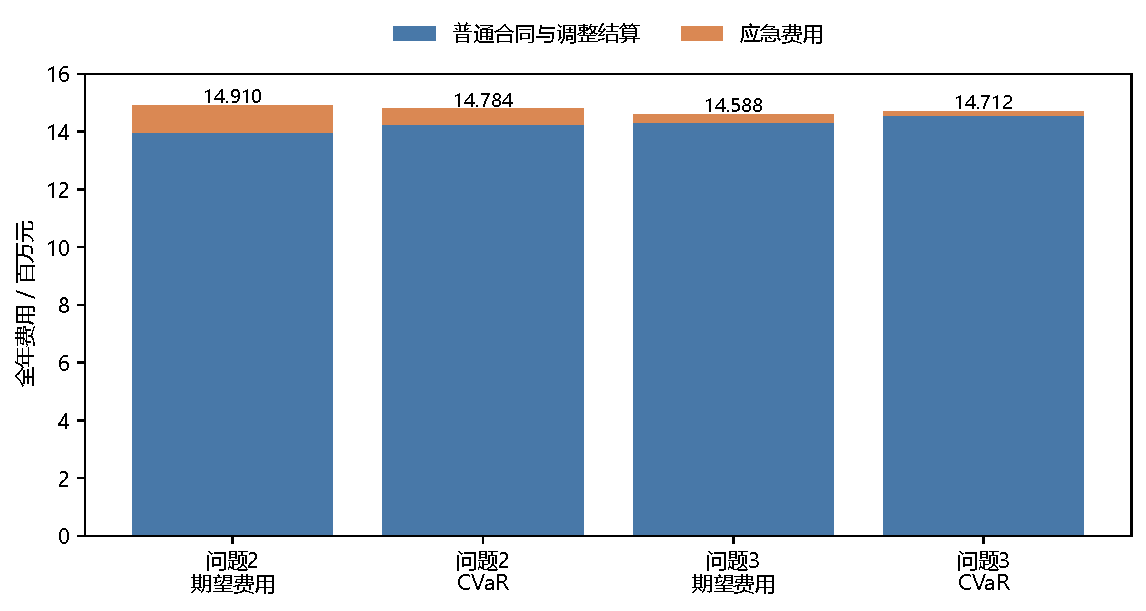
\includegraphics[width=\textwidth]{../figures/q4_cvar/cost_components.pdf}
        \caption*{(a) 四组策略全年电费构成拆解}
    \end{minipage}
    \hfill
    \begin{minipage}[t]{0.48\textwidth}
        \centering
        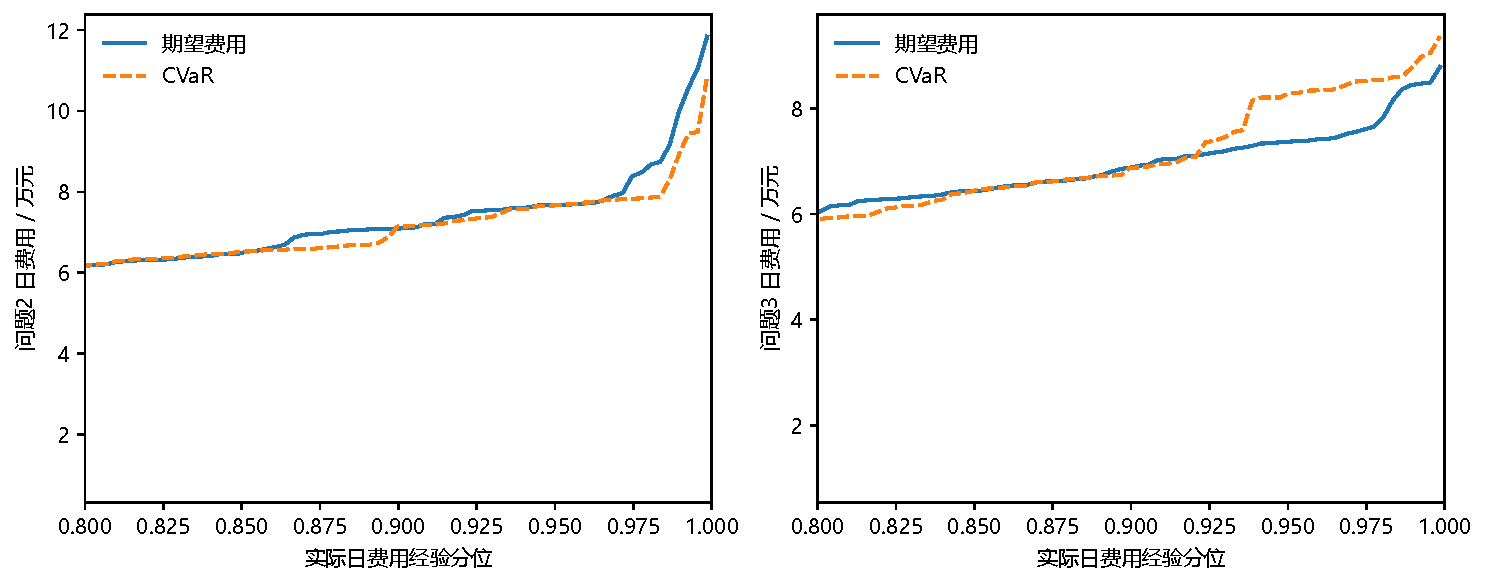
\includegraphics[width=\textwidth]{../figures/q4_cvar/daily_tail.pdf}
        \caption*{(b) 最贵 20\% 日期的尾部风险经验分布曲线}
    \end{minipage}
    \caption{波动电价下问题二与问题三策略的费用结构与尾部极端风险对比}
    \label{fig:q4_cost_tail}
\end{figure}

表 \ref{tab:q4_annual_comparison} 与图 \ref{fig:q4_cost_tail} 的结果可作如下解读：
\begin{enumerate}
    \item \textbf{问题二架构的样本内改善}：
    相较风险中性模型，CVaR 方案的全年总费用减少 $12.58$ 万元（$0.84\%$），实际最贵 $10\%$ 日的平均费用减少 $3.59\%$，紧急购电量由 $20.57$ 万 kWh 降至 $10.22$ 万 kWh。两组回退次数不同，不能将全部差异归因于 CVaR 项。
    
    \item \textbf{问题三架构的可比边界}：问题三的两组策略具有不同的回退次数，且与问题二的合同信息结构不同，因此不将两类策略的差异简单归因于滚动预报。问题三风险中性策略在本回测中的总费用最低，但这不是严格下界。
    
    \item \textbf{问题三中的风险--成本权衡}：加入 CVaR 后，紧急购电量降至 $4.17$ 万 kWh，但总费用增加 $12.49$ 万元（$+0.86\%$），实际日费用 CVaR$_{90}$ 也增加 $6.79\%$。该结果说明当前参数和有限历史场景下，风险项未改善该组样本外回测；其原因仍需独立实验验证。
\end{enumerate}

\subsection{四个指定日期的计算结果填报与调度解析}

\subsubsection{价格预测响应图谱}
图 \ref{fig:q4_price_forecast} 展示了在四个预先指定的典型日期（3月20日、6月21日、9月23日、12月21日）中，基于周滞后模型的 0:00 电价预测值与外网真实结算电价的时序拟合曲线。
\begin{figure}[htbp]
    \centering
    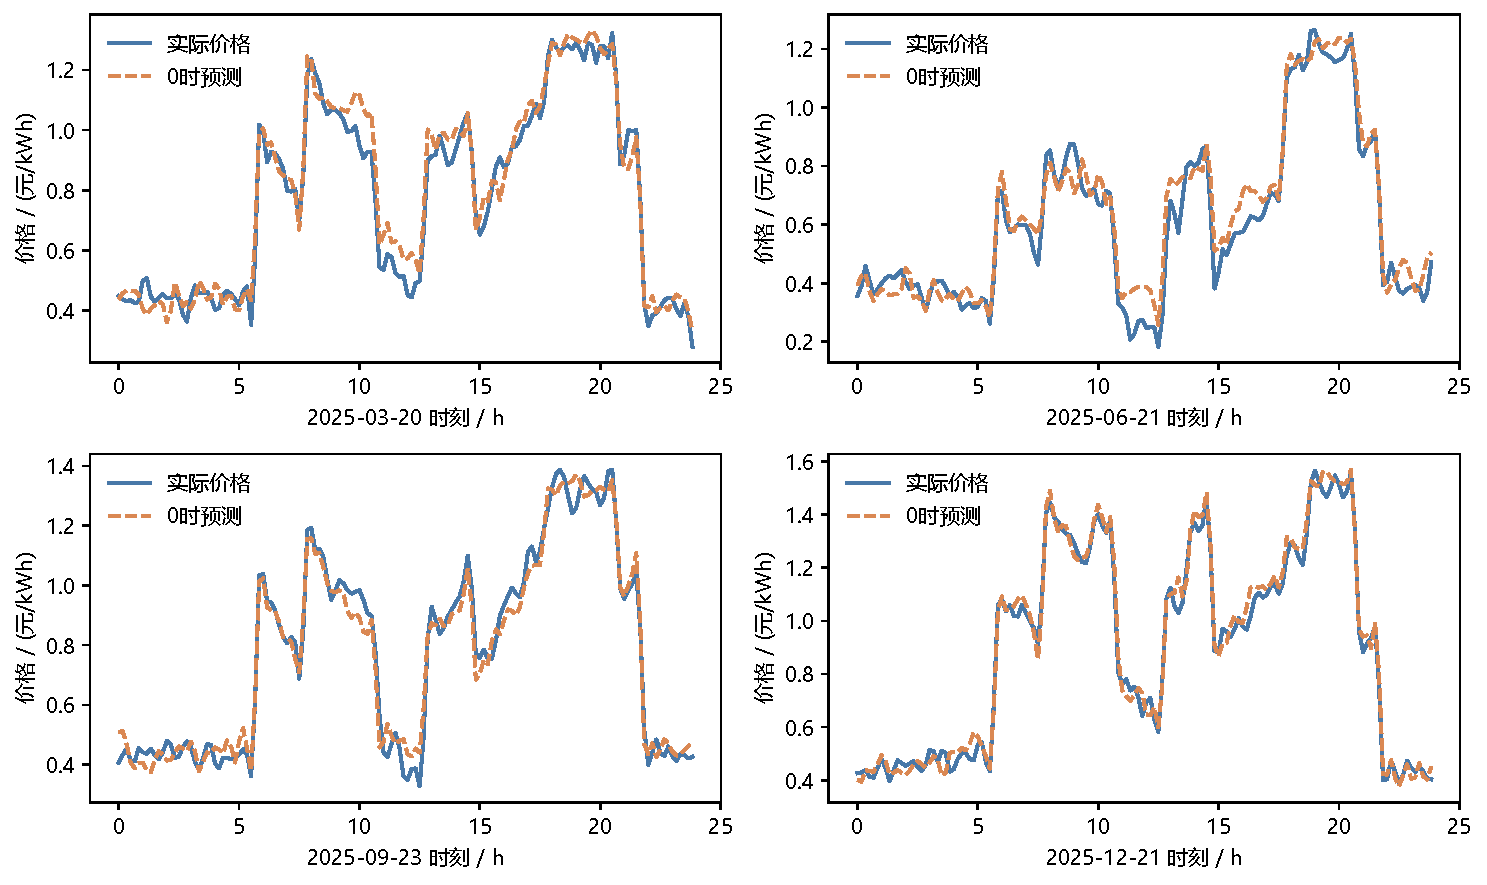
\includegraphics[width=0.92\textwidth]{../figures/q4_cvar/price_forecast.pdf}
    \caption{四个指定日期 0:00 外网电价预测值与日内真实结算电价时序拟合图}
    \label{fig:q4_price_forecast}
\end{figure}

图 \ref{fig:q4_price_forecast} 展示了四个预先指定日期的 0:00 价格预测与实际价格。周周期基准可反映部分日内结构，但预测误差仍通过联合场景进入后续优化，不能将该预测视为真实价格的精确复现。

\subsubsection{指定日期指标规范填报（result4-2 与 result4-3 关联汇总）}
表 \ref{tab:q4_specified_summary} 汇报四个指定日期在问题二和问题三策略下的关键指标；完整台账保存在 \texttt{results/q4\_cvar/} 对应策略目录。

\begin{table}[htbp]
\centering
\renewcommand{\arraystretch}{1.2}
\setlength{\tabcolsep}{4pt}
\caption{波动电价下四个指定日期在问题二与问题三 CVaR 策略下的关键运行与费用指标}
\label{tab:q4_specified_summary}
\begin{tabular*}{\textwidth}{@{\extracolsep{\fill}}llcccc@{}}
\toprule[1.5pt]
调度方案 & 统计指标维度 & 2025.3.20 & 2025.6.21 & 2025.9.23 & 2025.12.21 \\
\midrule[1pt]
\multirow{4}{*}{\textbf{问题二 CVaR}} 
  & 全天基础计划购电费 (元) & 42078.74 & 21134.73 & 49783.48 & 77410.44 \\
 & 全天紧急购电量 (kWh)     & $\approx 0.00$ & $0.00$ & $\approx 0.00$ & $\approx 0.00$ \\
  & 全天未利用电量 (kWh)   & 413.28  & 16696.41 & 4525.06  & 7313.86   \\
  & \textbf{全天实际总电费 (元)} & \textbf{42078.74} & \textbf{21134.73} & \textbf{49783.48} & \textbf{77410.44} \\
\midrule[0.5pt]
\multirow{4}{*}{\textbf{问题三 CVaR}} 
  & 0:00 基础计划费 (元) & 45943.59 & 20831.20 & 51089.40 & 82738.33 \\
  & 全天紧急购电量 (kWh)     & 0.00   & 0.00   & 0.00 & 583.04   \\
  & 全天紧急购电费用 (元)    & 0.00   & 0.00   & 0.00 & 1499.97  \\
  & \textbf{全天实际总电费 (元)} & \textbf{45163.37} & \textbf{19642.32} & \textbf{48125.65} & \textbf{84483.99} \\
\midrule[0.5pt]
\multicolumn{2}{l}{0:00 初态 / 24:00 末态 SOC (kWh)} & 2121 / 1672 & 3174 / 3696 & 3239 / 2911 & 1597 / 1671 \\
\bottomrule[1.5pt]
\end{tabular*}
\begin{tablenotes}
    \footnotesize
    \item \textbf{注}：问题三策略的 12 月 21 日包含一次回退，紧急购电量为 $583.04\text{ kWh}$。表中金额来自 \texttt{results/q4\_cvar/} 台账，未计入终端估值。
\end{tablenotes}
\end{table}

各指定日期的微网内部功率调度、紧急补电触发时刻与储能电池 SOC 联合响应如图 \ref{fig:q4_dispatch_soc} 所示。
\begin{figure}[htbp]
    \centering
    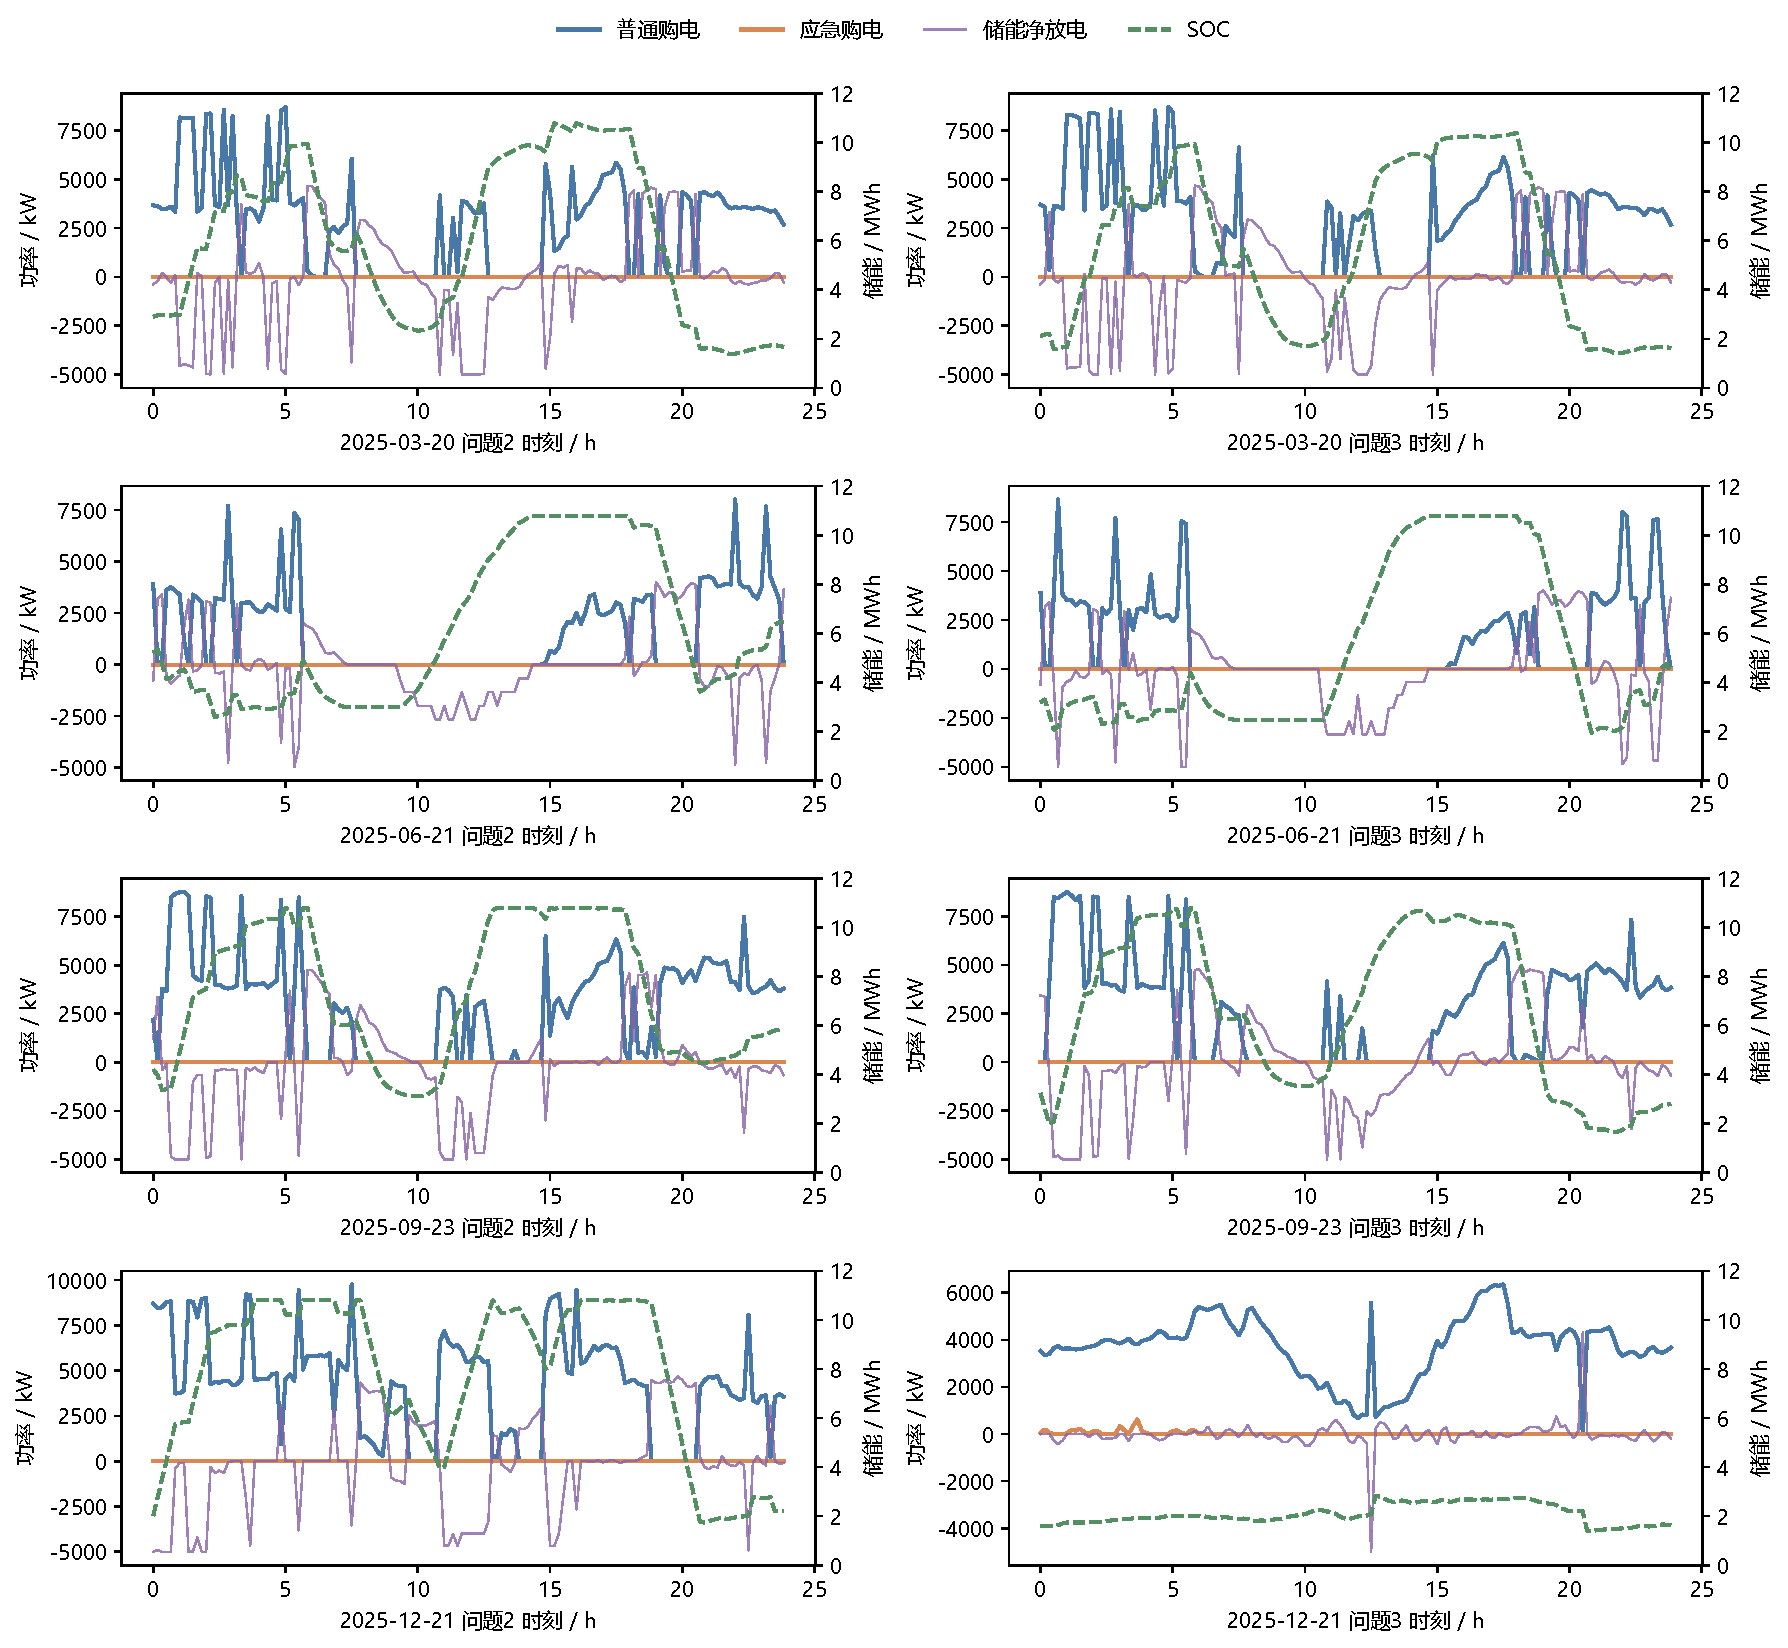
\includegraphics[width=0.96\textwidth]{../figures/q4_cvar/dispatch_soc.pdf}
    \caption{波动电价下四个指定日期在问题二与问题三模式下的功率调度与电池 SOC 演化响应}
    \label{fig:q4_dispatch_soc}
\end{figure}

从图 \ref{fig:q4_dispatch_soc} 可以观察到：在部分指定日期中，储能在光伏富余或低价时段充电，在高价时段放电；但不同策略和日期的 SOC 轨迹并不相同，不能据此概括为所有时段均达到 $10800\text{ kWh}$ 或实现全局最优。
% =========================================================================
%                               模型的评价、改进与推广
% =========================================================================
\section{模型的评价、改进与推广}

\subsection{模型的优点}
\begin{enumerate}
    \item \textbf{理论严谨性}：严格证明了充放电互斥性在 LP 松弛下的自然满足，大幅提升了多时段大规模调度的求解速度。
    \item \textbf{因果防穿越设计}：预测与日前决策严格杜绝任何未来信息泄露，符合实际工程闭环运行环境。
    \item \textbf{精细化台账管理}：能量平衡与经济结算具有完备的逐段台账支持，残差均处于计算机浮点误差极值。
\end{enumerate}

\subsection{模型的局限性与改进方向}
\begin{enumerate}
    \item \textbf{电池老化成本折损}：未考虑电池频繁循环引起的容量衰退衰减机理，未来可引入电池退化折旧惩罚项。
    \item \textbf{电网潮流约束}：简化了线路阻抗与节点电压损耗，后续可与 AC-OPF（交流最优潮流）结合拓展。
\end{enumerate}

\subsection{模型的推广应用前景}
本文提出的分层控制律与日前申报方法，可平滑移植到工业园区微电网、光储充一体化充电站以及虚拟电厂（VPP）参与电力现货市场的实际运营中。


% =========================================================================
%                         AI 工具使用声明（2026 年新规）
% 规则：必须放置在【参考文献之前】！
% =========================================================================

\CumcmAIUsed{本参赛队在竞赛过程中使用了 AI 工具，主要用于论文语言润色、绘图脚本语法排查、LaTeX 排版格式自检和代码规范性核验；核心数学模型、算法设计、计算运行及结果分析由参赛队完成并人工复核，详细使用情况见支撑材料。}


% =========================================================================
%                               参考文献
% 严格遵循真实发表学术文献（涵盖储能经济调度、两阶段优化、MPC、CVaR）
% =========================================================================
\begin{thebibliography}{99}
    \bibitem{bib:format} 全国大学生数学建模竞赛组委会. 全国大学生数学建模竞赛论文格式规范[EB/OL]. 2026.
    \bibitem{bib:liu} 刘海洋. \LaTeX{} 入门[M]. 北京: 电子工业出版社, 2013.
    \bibitem{bib:rockafellar} ROCKAFELLAR R T, URYASEV S. Optimization of conditional value-at-risk[J]. Journal of Risk, 2000, 2(3): 21-41.
    \bibitem{bib:pacaud} PACAUD F, CARPENTIER P, CHANCELIER J P, et al. Optimization of a domestic microgrid equipped with solar panel and battery: model predictive control and stochastic dual dynamic programming approaches[J]. Energy Systems, 2024, 15(1): 115-139.
    \bibitem{bib:zheng} 郑漳华, 艾芊. 微电网的研究现状及在我国的应用前景[J]. 电网技术, 2008, 32(16): 27-31.
    \bibitem{bib:zhou} 周步祥, 邹佳辉, 董申, 等. 基于共享储能的微网园区系统能量协同优化[J]. 电气传动, 2021, 51(18): 69-74.
    \bibitem{bib:xu} 徐艳春, 刘海权, 孙思涵, 等. 计及需求响应和共享储能的多微网系统双层优化调度[J]. 电力自动化设备, 2023, 43(6): 135-141.
    \bibitem{bib:wu} 吴斌丰, 傅莹, 陈杨哲, 等. 考虑紧急备用与光伏出力不确定性的微电网分布式储能规划方法[J]. 浙江电力, 2021, 40(9): 32-40.
    \bibitem{bib:zhang} 张祥宇, 舒意南, 付媛, 等. 含虚拟储能直流微电网的源荷储能量协同优化控制[J]. 中国电机工程学报, 2021, 41(15): 5214-5226.
\end{thebibliography}

% =========================================================================
%                               附录部分
% =========================================================================
\clearpage
\begin{appendices}

% ==================== 附录 A：文件与成果交付清单 ====================
\section{支撑材料与成果交付文件列表}

本参赛队的所有计算结果均通过独立脚本生成并经全量物理约束核验，完整的程序源码、求解台账与结果工作簿均保存在支撑材料中，文件结构与功能如表 \ref{tab:app_files} 所示。

\begin{table}[htbp]
\centering
\small
\renewcommand{\arraystretch}{1.25}
\caption{支撑材料核心文件与交付成果清单}
\label{tab:app_files}
\begin{tabular*}{\textwidth}{p{0.26\textwidth} p{0.14\textwidth} p{0.54\textwidth}}
\toprule[1.5pt]
目录/文件名 & 文件类型 & 功能描述与内容定义 \\
\midrule[1pt]
\textbf{AI工具使用详情.pdf} & PDF 文档 & 按 2026 年竞赛要求另行提交的 AI 工具使用过程与人工核验说明 \\
\textbf{result1.xlsx}       & 结果表格 & 问题一在 0:00 制定的全天 144 个时段计划购电与 4 小时充放电最终结果 \\
\textbf{result2.xlsx}       & 结果表格 & 问题二正式期（334 天）计划购电量、充放电量及紧急购电时段明细 \\
\textbf{result3.xlsx}       & 结果表格 & 问题三正式期基准计划购电量、滚动调整购电量、充放电及紧急购电量 \\
\texttt{results/q4_cvar/q2_cvar/} & 结果目录 & 问题四问题二架构 CVaR 策略的逐日合同、台账与验收文件 \\
\texttt{results/q4_cvar/q3_cvar/} & 结果目录 & 问题四问题三架构 CVaR 策略的逐日合同、台账与验收文件 \\
\midrule[0.5pt]
\texttt{solve\_c\_q1\_pilot.py}    & Python 源码 & 问题一多时段经济调度 LP/MILP 快速求解算法与参数敏感性测试 \\
\texttt{solve\_c\_q2\_enhanced.py} & Python 源码 & 问题二历史因果预测择优、分位数安全余量与 48h 滚动前瞻优化算法 \\
\texttt{run\_c\_q3\_tree.py}       & Python 源码 & 问题三四阶段场景树构建、非对称摩擦结算与滚动 MPC 控制算法 \\
\texttt{run\_c\_q4\_cvar.py}       & Python 源码 & 问题四负荷--光伏--电价三维联合场景生成与均值--CVaR 鲁棒求解程序 \\
\texttt{verify\_c\_q2\_enhanced.py}、\texttt{verify\_c\_q3\_tree.py} & Python 源码 & 对应策略的母线守恒、SOC 递推、功率和互斥性验收脚本 \\
\bottomrule[1.5pt]
\end{tabular*}
\end{table}
\normalsize

% ==================== 附录 B：核心算法实现源码 ====================
\section{核心算法实现源码清单}

\subsection{问题一：基于 LP 松弛的经济调度求解算法 (Python)}
\begin{lstlisting}[language=python]
import numpy as np
from scipy.optimize import linprog

def solve_q1_deterministic(price, load, pv, eta_c=0.9, eta_d=0.9, E0=6000.0):
    # 问题一线性规划求解函数；结果需通过充放电互斥性复核
    T = len(price)
    M = 5000.0 / 6.0  # 10分钟单时段最大充放电量限制 (kWh)
    
    # 决策变量排列: q(0:T), c(T:2T), d(2T:3T), s(3T:4T), E(4T:5T+1)
    n_vars = 5 * T + 1
    c_obj = np.zeros(n_vars)
    c_obj[:T] = price  # 优化目标: 最小化购电电费
    
    A_eq = []
    b_eq = []
    
    # 构建各时段母线平衡与电池SOC递推等式
    for t in range(T):
        # 母线功率平衡: q_t - c_t + d_t - s_t = L_t - V_t
        row_bal = np.zeros(n_vars)
        row_bal[t] = 1.0
        row_bal[T + t] = -1.0
        row_bal[2*T + t] = 1.0
        row_bal[3*T + t] = -1.0
        A_eq.append(row_bal)
        b_eq.append(load[t] - pv[t])
        
        # 储能状态转移方程: E_{t+1} - E_t - 0.9*c_t + d_t/0.9 = 0
        row_soc = np.zeros(n_vars)
        row_soc[4*T + t + 1] = 1.0
        row_soc[4*T + t] = -1.0
        row_soc[T + t] = -eta_c
        row_soc[2*T + t] = 1.0 / eta_d
        A_eq.append(row_soc)
        b_eq.append(0.0)
        
    # 日初与日末电量平衡约束: E_0 = E_144 = 6000 kWh
    r_start = np.zeros(n_vars); r_start[4*T] = 1.0; A_eq.append(r_start); b_eq.append(E0)
    r_end = np.zeros(n_vars); r_end[4*T + T] = 1.0; A_eq.append(r_end); b_eq.append(E0)
    
    # 变量物理边界设置
    bounds = []
    for t in range(T): bounds.append((0, None))             # 购电量非负
    for t in range(T): bounds.append((0, M))                # 充电功率上限
    for t in range(T): bounds.append((0, M))                # 放电功率上限
    for t in range(T): bounds.append((0, None))             # 弃电量非负
    for t in range(T + 1): bounds.append((1200.0, 10800.0)) # 电池安全容量区间
    
    # 调用 HiGHS 单纯形法求解器
    res = linprog(c_obj, A_eq=np.array(A_eq), b_eq=np.array(b_eq), 
                  bounds=bounds, method='highs-ds')
    return res
\end{lstlisting}

\subsection{问题二：分位数安全余量生成与因果日前规划算法 (Python)}
\begin{lstlisting}[language=python]
import numpy as np

def compute_quantile_margins(history_residuals, alpha=0.8):
    # 根据过去28天的净负荷真实残差，计算时变80分位数非负安全余量
    # 输入矩阵形状为 (28天, 144时段)
    percentile_target = alpha * 100.0
    q_val = np.percentile(history_residuals, percentile_target, axis=0)
    
    # 截断非负值，确立各时段安全防护边际
    margin = np.maximum(0.0, q_val)
    return margin

def solve_q2_day_ahead_plan(price_curve, load_pred, pv_pred, margin, E_start):
    # 48小时跨日前瞻优化: 输入叠加安全余量后的用电需求
    H = 288  # 48小时对应288个10分钟时段
    
    # 拼接日前与虚拟次日前瞻序列
    ext_load = np.concatenate([load_pred + margin, load_pred + margin])
    ext_pv = np.concatenate([pv_pred, pv_pred])
    ext_price = np.concatenate([price_curve, price_curve])
    
    # 引入末端连续蓄能惩罚项 lambda = min(price) / 0.9 求解MILP
    # 执行刚性申报规则: 仅截取并冻结前144时段作为当天计划购电量
    # 后144时段仅作前瞻引导，次日重新滚动优化
    pass
\end{lstlisting}

\subsection{问题四：Rockafellar-Uryasev CVaR 风险约束线性化建模 (Python)}
\begin{lstlisting}[language=python]
def build_cvar_objective(scenarios_cost, beta=0.20, alpha=0.90):
    # CVaR 风险指标线性规划构建
    # 目标函数: (1 - beta)*E[C] + beta*[ zeta + (1/(1-alpha))*sum(p_w * xi_w) ]
    # 约束条件: xi_w >= C_w - zeta, xi_w >= 0
    N_omega = len(scenarios_cost)
    prob = 1.0 / N_omega
    
    # 引入辅助决策标量 zeta 以及各联合场景超额损失变量 xi
    # 权衡期望电费收益与最贵10个百分点极端日的尾部在险损失
    pass
\end{lstlisting}

\end{appendices}
\end{document}
